\documentclass[12pt,a4paper]{article}

% --- Packages ---
\usepackage[utf8]{inputenc}
\usepackage[T1]{fontenc}
\usepackage{helvet}
\renewcommand{\familydefault}{\sfdefault}
\usepackage[margin=2.5cm]{geometry}
\usepackage{graphicx}
\usepackage{booktabs}
\usepackage{array}
\usepackage{multirow}
\usepackage{hyperref}
\usepackage{xcolor}
\usepackage{float}
\usepackage{enumitem}
\usepackage{caption}
\usepackage{subcaption}
\usepackage{amsmath}
\usepackage{fancyhdr}
\usepackage{titlesec}
\usepackage{parskip}

% --- Colors ---
\definecolor{sectionblue}{HTML}{2C3E50}
\definecolor{linkblue}{HTML}{2980B9}
\definecolor{bearish}{HTML}{E74C3C}
\definecolor{bullish}{HTML}{2ECC71}
\definecolor{neutral}{HTML}{3498DB}

% --- Hyperref setup ---
\hypersetup{
    colorlinks=true,
    linkcolor=sectionblue,
    urlcolor=linkblue,
    citecolor=sectionblue,
}

% --- Section formatting ---
\titleformat{\section}{\Large\bfseries\color{sectionblue}}{}{0em}{}[\titlerule]
\titleformat{\subsection}{\large\bfseries\color{sectionblue!80}}{}{0em}{}
\titleformat{\subsubsection}{\normalsize\bfseries\color{sectionblue!60}}{}{0em}{}
\titlespacing*{\section}{0pt}{18pt}{8pt}
\titlespacing*{\subsection}{0pt}{12pt}{4pt}

% --- Header/Footer ---
\pagestyle{fancy}
\fancyhf{}
\fancyhead[L]{\small\color{gray}Group 42 --- Text Mining 2025/2026}
\fancyhead[R]{\small\color{gray}NOVA IMS}
\fancyfoot[C]{\thepage}
\renewcommand{\headrulewidth}{0.4pt}

% --- Figure path ---
\graphicspath{{../figures/}}

% --- Caption style ---
\captionsetup{font=small, labelfont=bf, skip=6pt}

\begin{document}

% ============================================================================
% TITLE PAGE
% ============================================================================
\begin{titlepage}
\centering
\vspace*{2cm}
{\Huge\bfseries Financial Tweet\\[6pt] Sentiment Classification\par}
\vspace{1.5cm}
{\LARGE Group 42\par}
\vspace{0.5cm}
{\Large Text Mining 2025/2026\par}
{\Large NOVA Information Management School\par}
\vspace{2cm}
\begin{tabular}{ll}
\toprule
\textbf{Name} & \textbf{Student ID} \\
\midrule
TBD & TBD \\
TBD & TBD \\
TBD & TBD \\
TBD & TBD \\
\bottomrule
\end{tabular}
\vfill
{\large \today\par}
\end{titlepage}

% ============================================================================
% TABLE OF CONTENTS
% ============================================================================
\tableofcontents
\newpage

% ============================================================================
% 1. INTRODUCTION
% ============================================================================
\section{Introduction}

This report presents a systematic approach to classifying financial tweets as \textbf{Bearish}~(0), \textbf{Bullish}~(1), or \textbf{Neutral}~(2). Financial sentiment analysis on social media has practical applications in algorithmic trading, market surveillance, and investor sentiment tracking. The challenge lies in the brevity and informality of tweets, domain-specific vocabulary (cashtags, financial jargon), and inherent class imbalance where neutral commentary dominates.

We evaluate \textbf{32 combinations} of feature extraction methods and classifiers using 5-fold stratified cross-validation, with macro-F1 as the primary metric. Our best pipeline --- \textbf{Twitter-RoBERTa embeddings + XGBoost} --- achieves a macro-F1 of \textbf{0.794}.

% ============================================================================
% 2. DATA EXPLORATION
% ============================================================================
\section{Data Exploration}

\subsection{Dataset Overview}

The dataset consists of \textbf{9,543 training tweets} and \textbf{2,388 test tweets}, each labeled with one of three sentiment classes.

\begin{table}[H]
\centering
\caption{Training set class distribution.}
\label{tab:class_dist}
\begin{tabular}{lrr}
\toprule
\textbf{Class} & \textbf{Count} & \textbf{Proportion} \\
\midrule
Bearish (0) & 1,442 & 15.1\% \\
Bullish (1) & 1,923 & 20.1\% \\
Neutral (2) & 6,178 & 64.7\% \\
\bottomrule
\end{tabular}
\end{table}

The dataset exhibits significant class imbalance --- Neutral tweets outnumber Bearish tweets by a factor of 4.3$\times$. This motivates two key design decisions: (1)~using \texttt{class\_weight='balanced'} in all classifiers to prevent majority-class bias, and (2)~adopting macro-F1 as the primary metric rather than accuracy, since a naive all-Neutral classifier would achieve 64.7\% accuracy while failing completely on minority classes.

\begin{figure}[H]
\centering
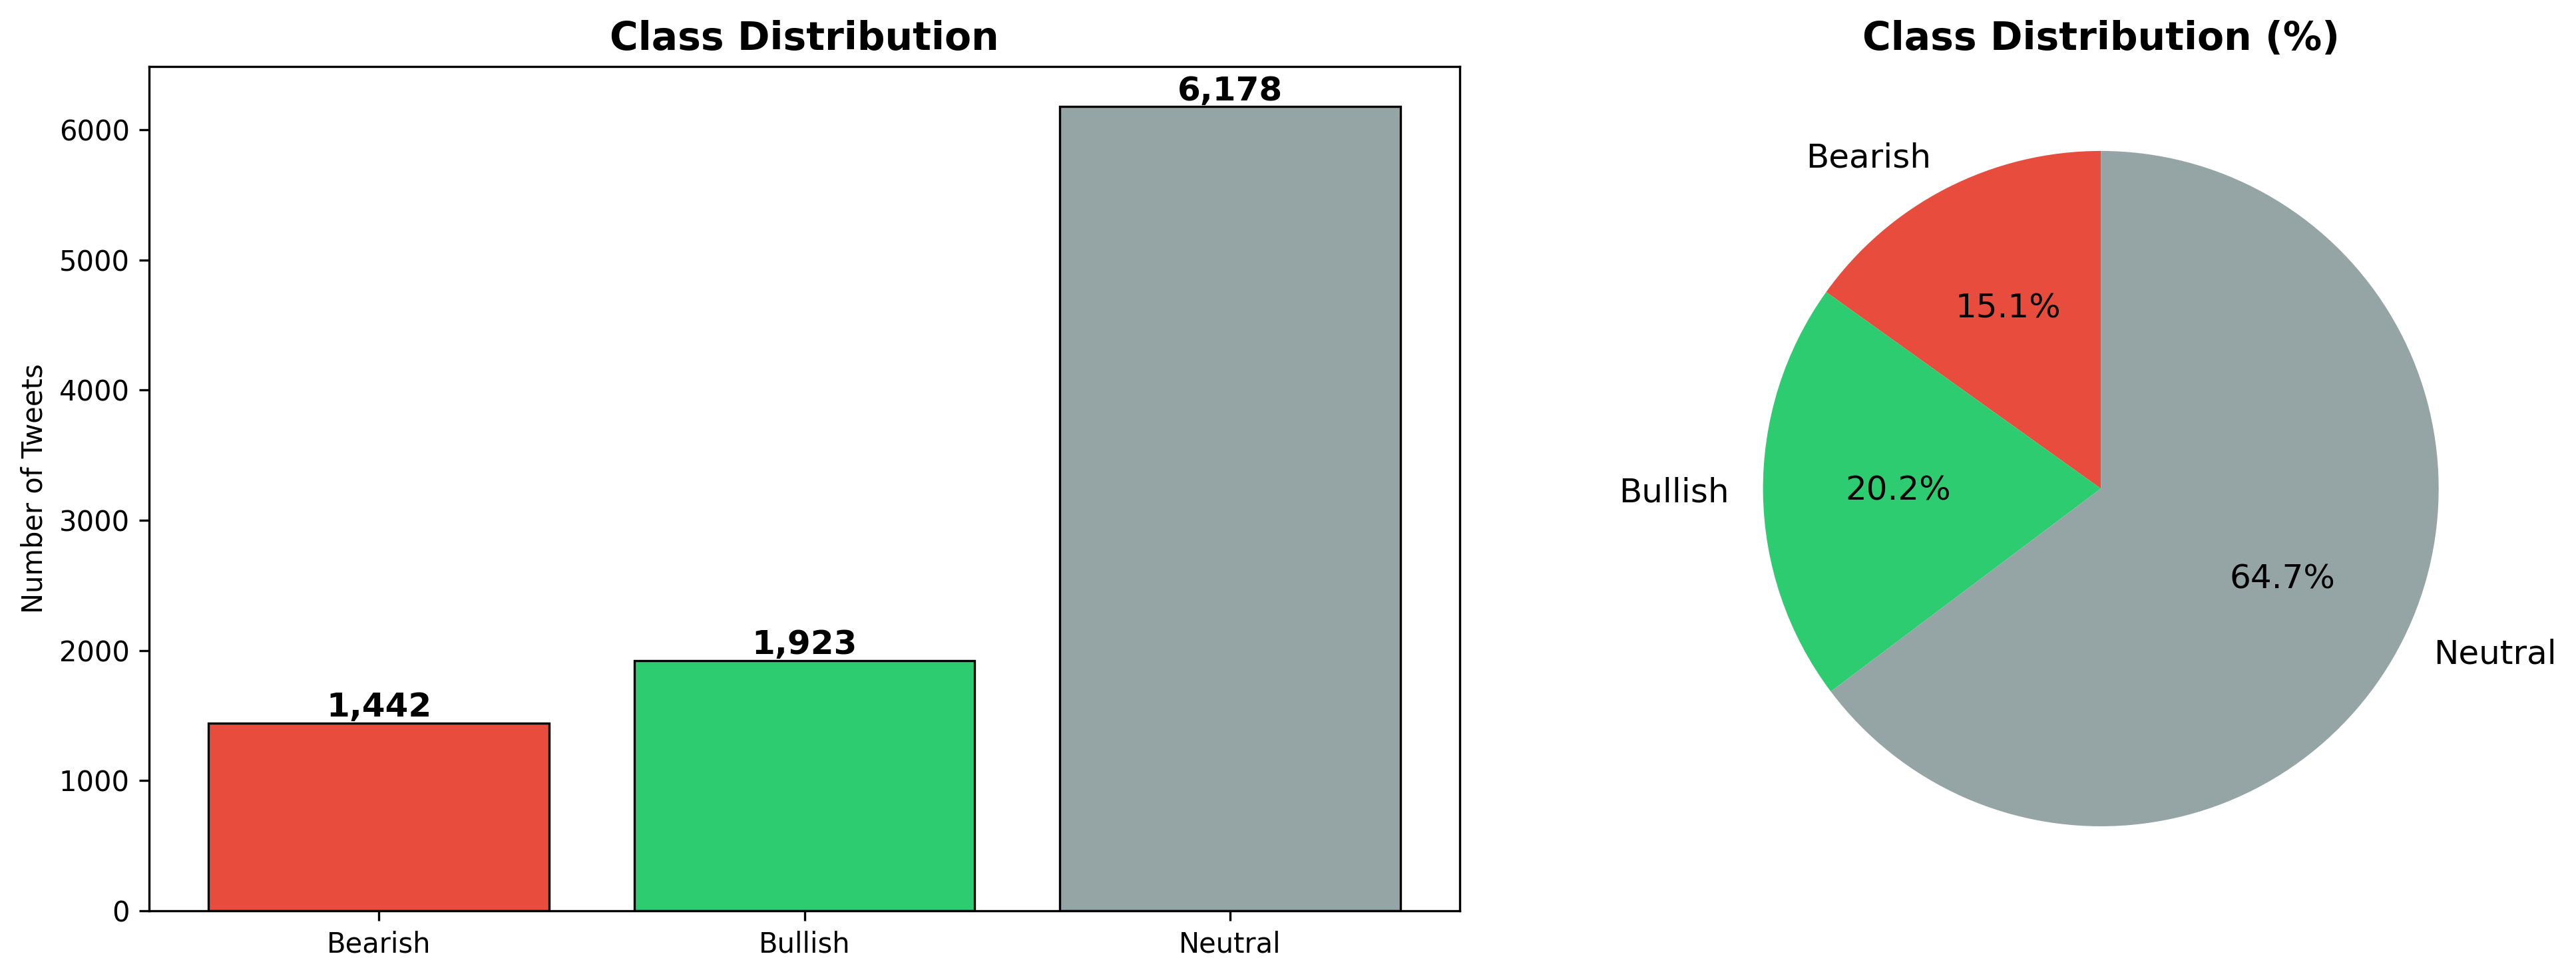
\includegraphics[width=0.85\textwidth]{class_distribution.png}
\caption{Class distribution in the training set, showing significant imbalance toward Neutral.}
\label{fig:class_dist}
\end{figure}

\subsection{Tweet Characteristics}

Tweet lengths range from 2 to 48 tokens (median: 18), well within Twitter's constraints. All three classes show similar length distributions, indicating that length alone is not discriminative. This also justifies using \texttt{max\_length=128} for Transformer tokenization --- no tweet approaches this limit.

\begin{figure}[H]
\centering
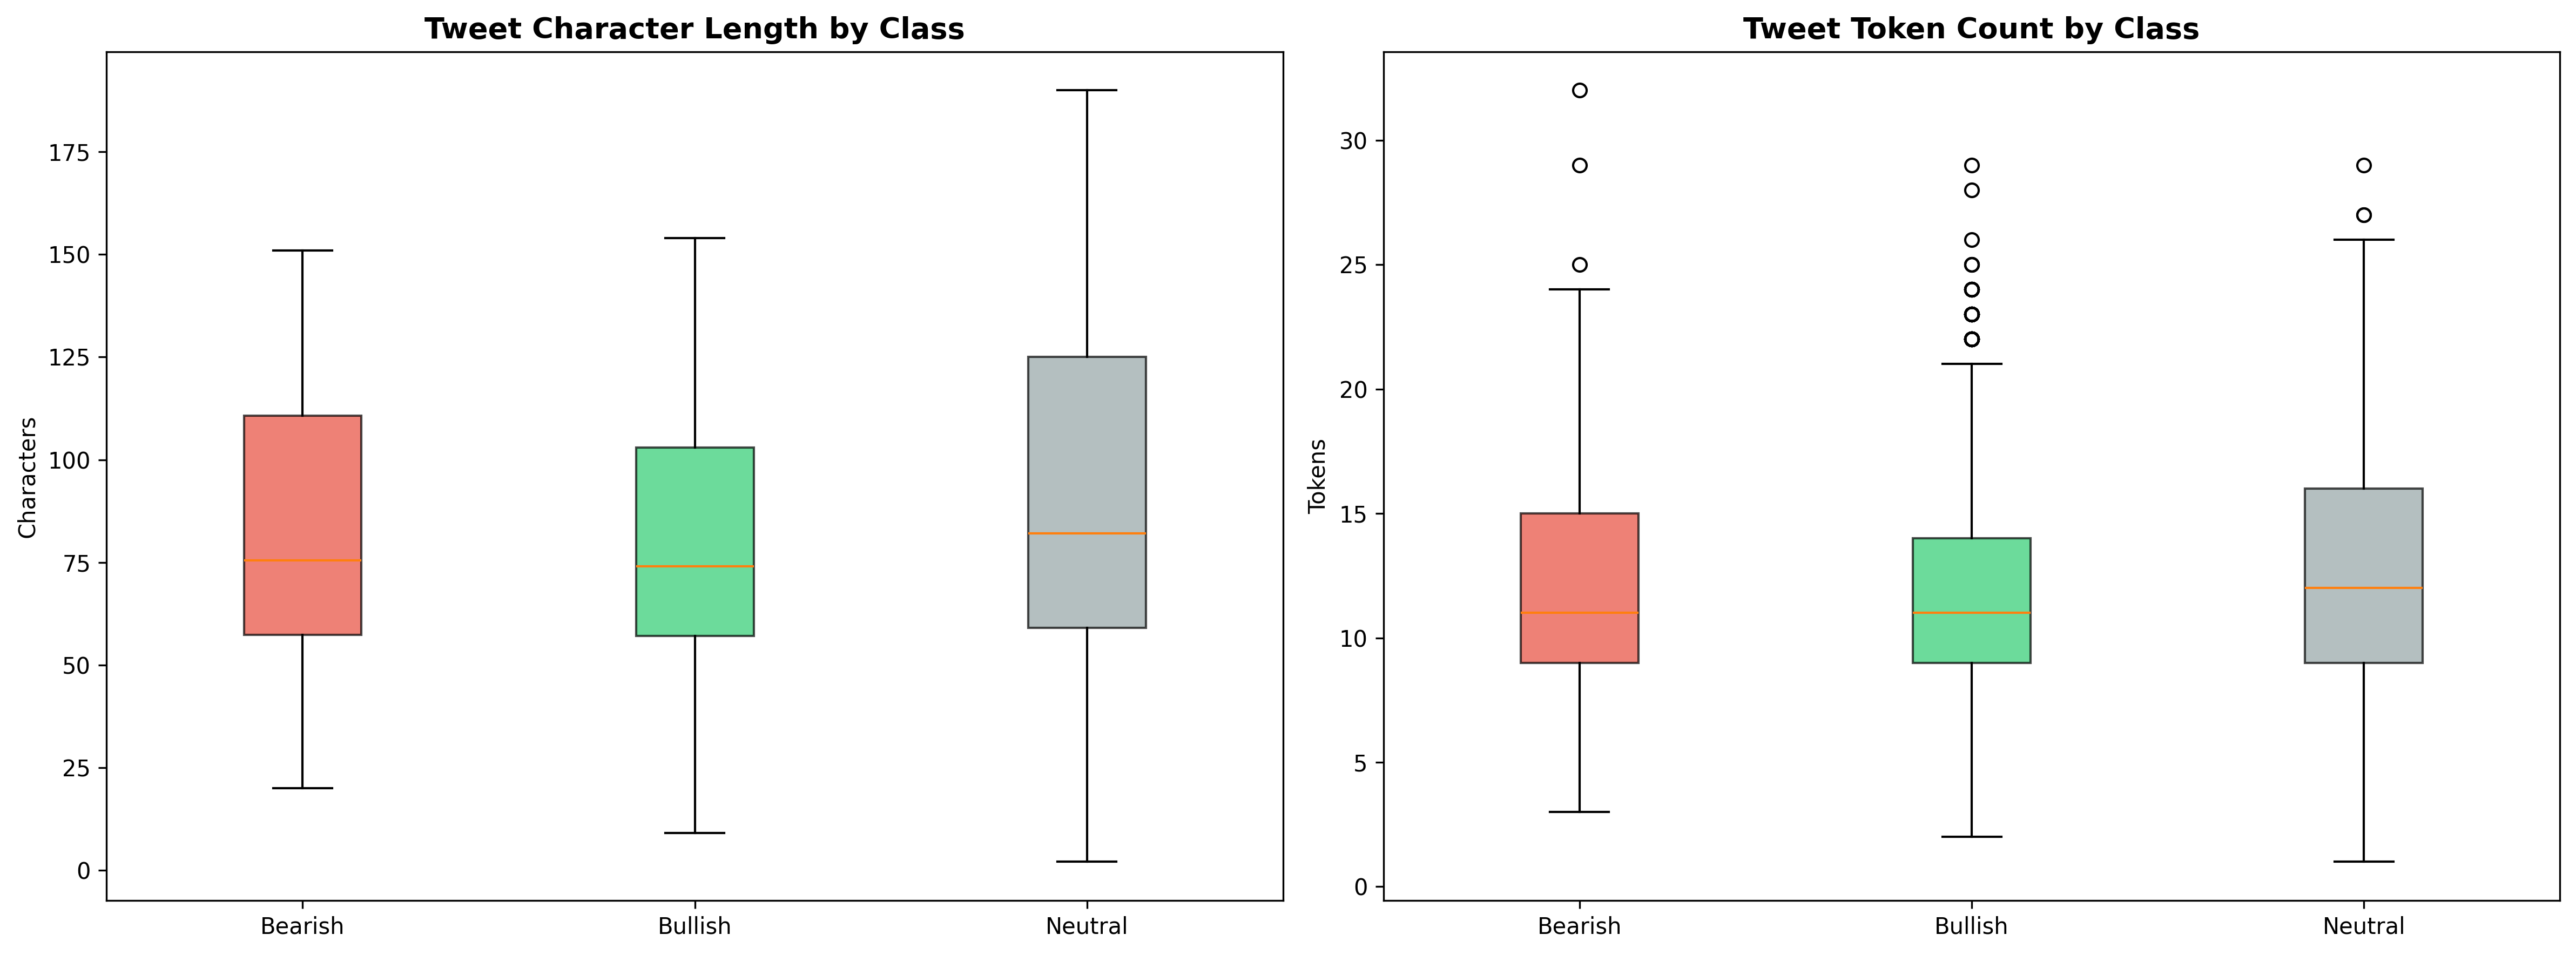
\includegraphics[width=0.85\textwidth]{tweet_length_distribution.png}
\caption{Tweet length distribution (characters and tokens) across sentiment classes.}
\label{fig:tweet_length}
\end{figure}

\subsection{Domain-Specific Features}

Financial tweets contain distinctive markers:

\begin{itemize}[nosep]
    \item \textbf{\$TICKER cashtags} (e.g., \$AAPL, \$TSLA): Present in ${\sim}60\%$ of tweets. We replace them with a \texttt{<TICKER>} placeholder to preserve signal without overfitting to specific stock names.
    \item \textbf{@mentions}: Present in ${\sim}15\%$ of tweets; removed as they carry no sentiment signal.
    \item \textbf{URLs}: Present in ${\sim}20\%$ of tweets; removed as they point to unavailable external content.
    \item \textbf{Hashtags}: The \texttt{\#} symbol is stripped but the word is retained (e.g., \texttt{\#bullish} $\rightarrow$ \texttt{bullish}).
\end{itemize}

\begin{figure}[H]
\centering
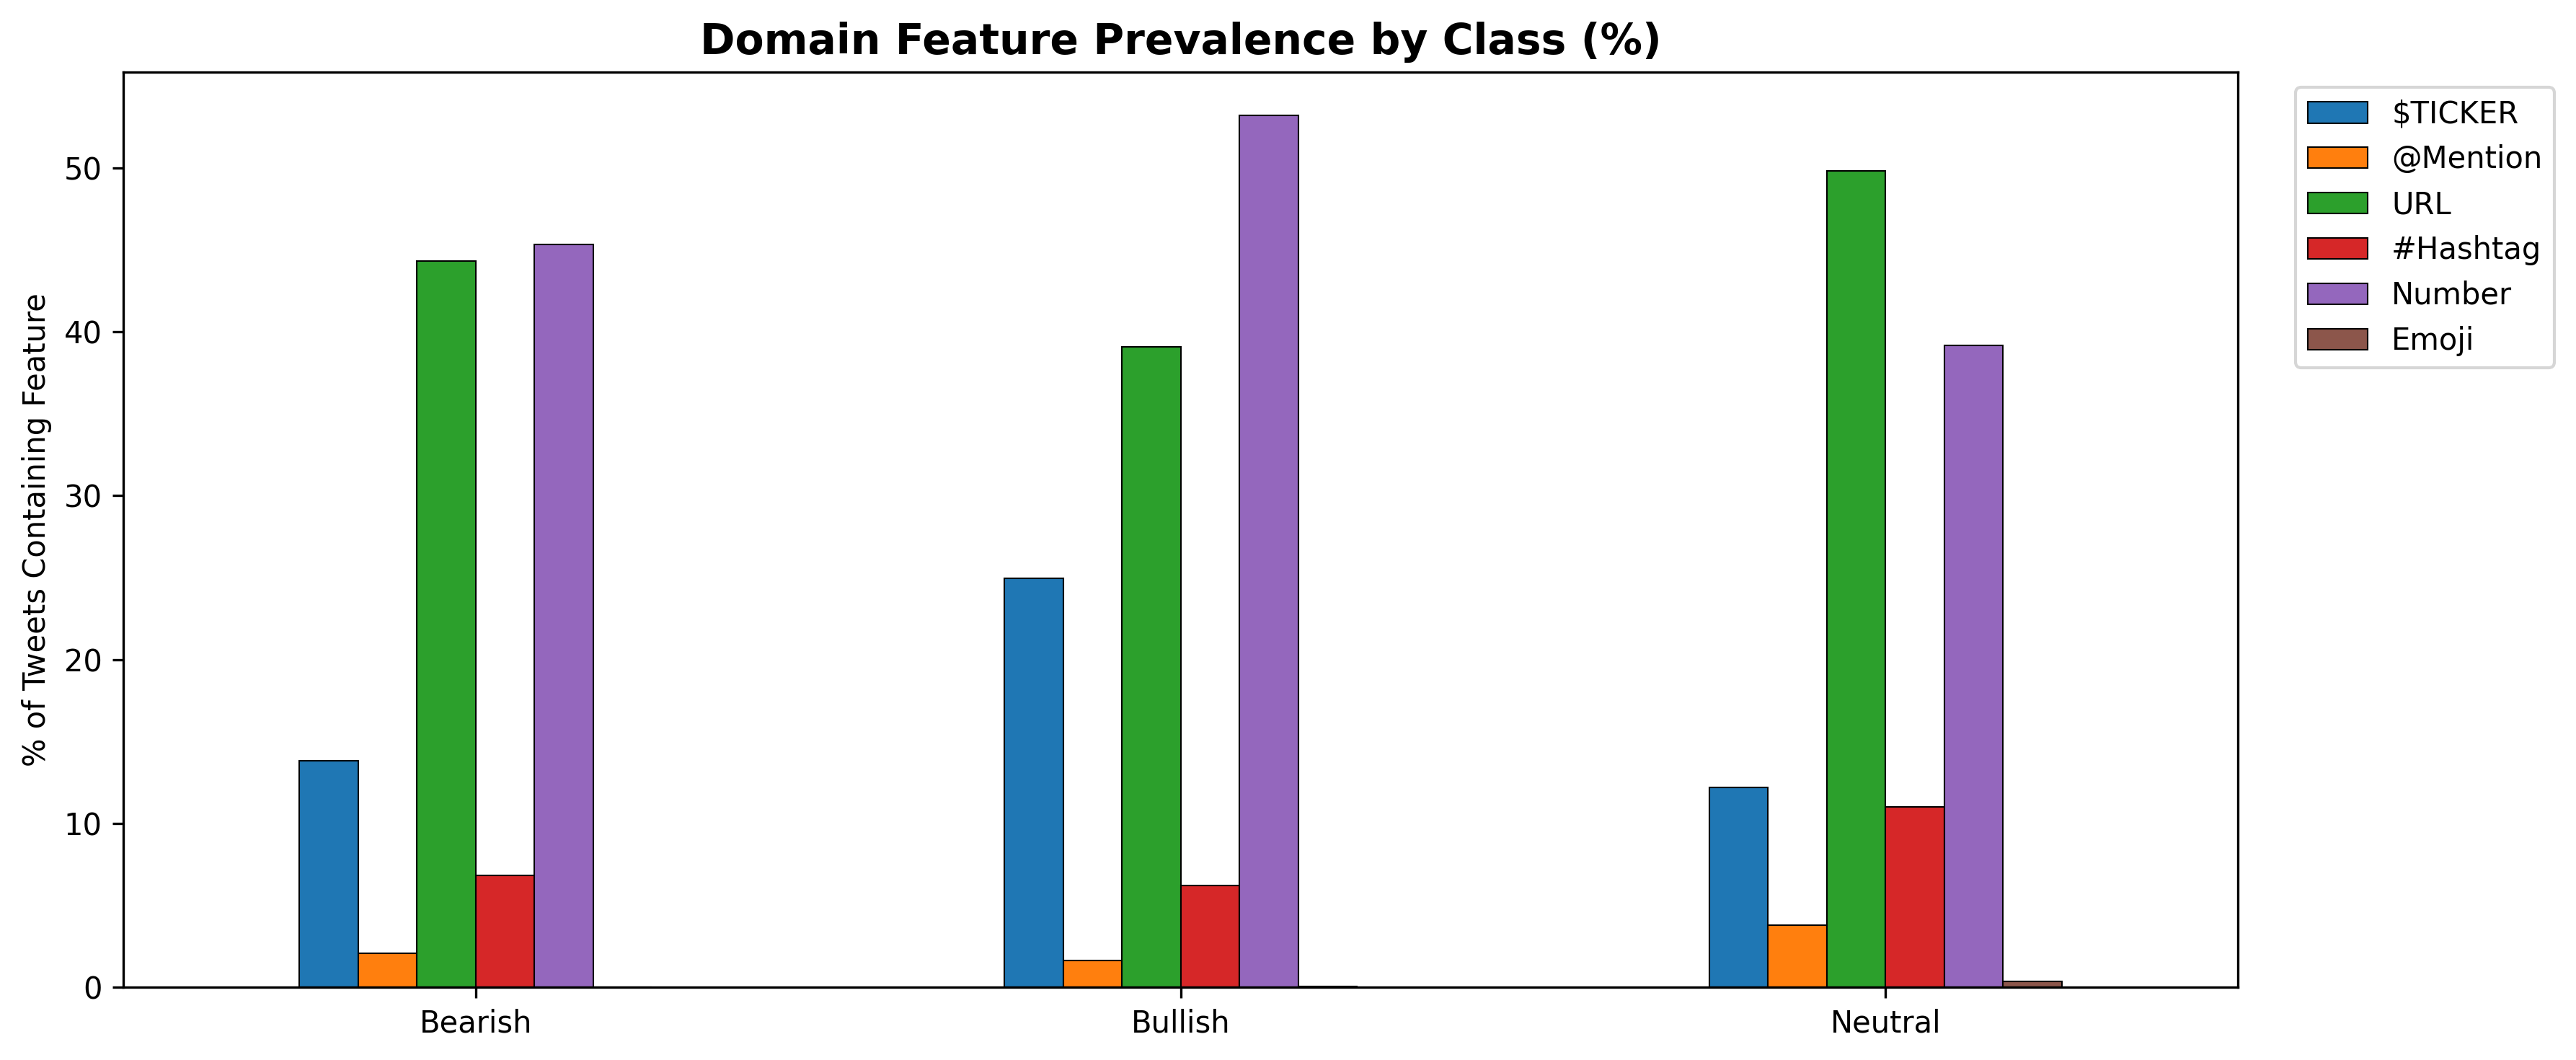
\includegraphics[width=0.85\textwidth]{domain_features.png}
\caption{Prevalence of domain-specific features across sentiment classes.}
\label{fig:domain_features}
\end{figure}

\subsection{Discriminative Vocabulary}

Analysis of top tokens per class reveals clear thematic separation:

\begin{itemize}[nosep]
    \item \textbf{\textcolor{bearish}{Bearish}}: ``cut'', ``downgrade'', ``sell'', ``loss'', ``short'', ``crash'', ``bear''
    \item \textbf{\textcolor{bullish}{Bullish}}: ``buy'', ``upgrade'', ``breakout'', ``moon'', ``bull'', ``long'', ``growth''
    \item \textbf{\textcolor{neutral}{Neutral}}: ``earnings'', ``report'', ``market'', ``stock'', ``today'', ``trade''
\end{itemize}

The Neutral class vocabulary overlaps significantly with both Bearish and Bullish, confirming that Neutral is the hardest class to discriminate --- it acts as a catch-all for informational tweets without explicit sentiment.

\begin{figure}[H]
\centering
\begin{subfigure}[t]{0.48\textwidth}
    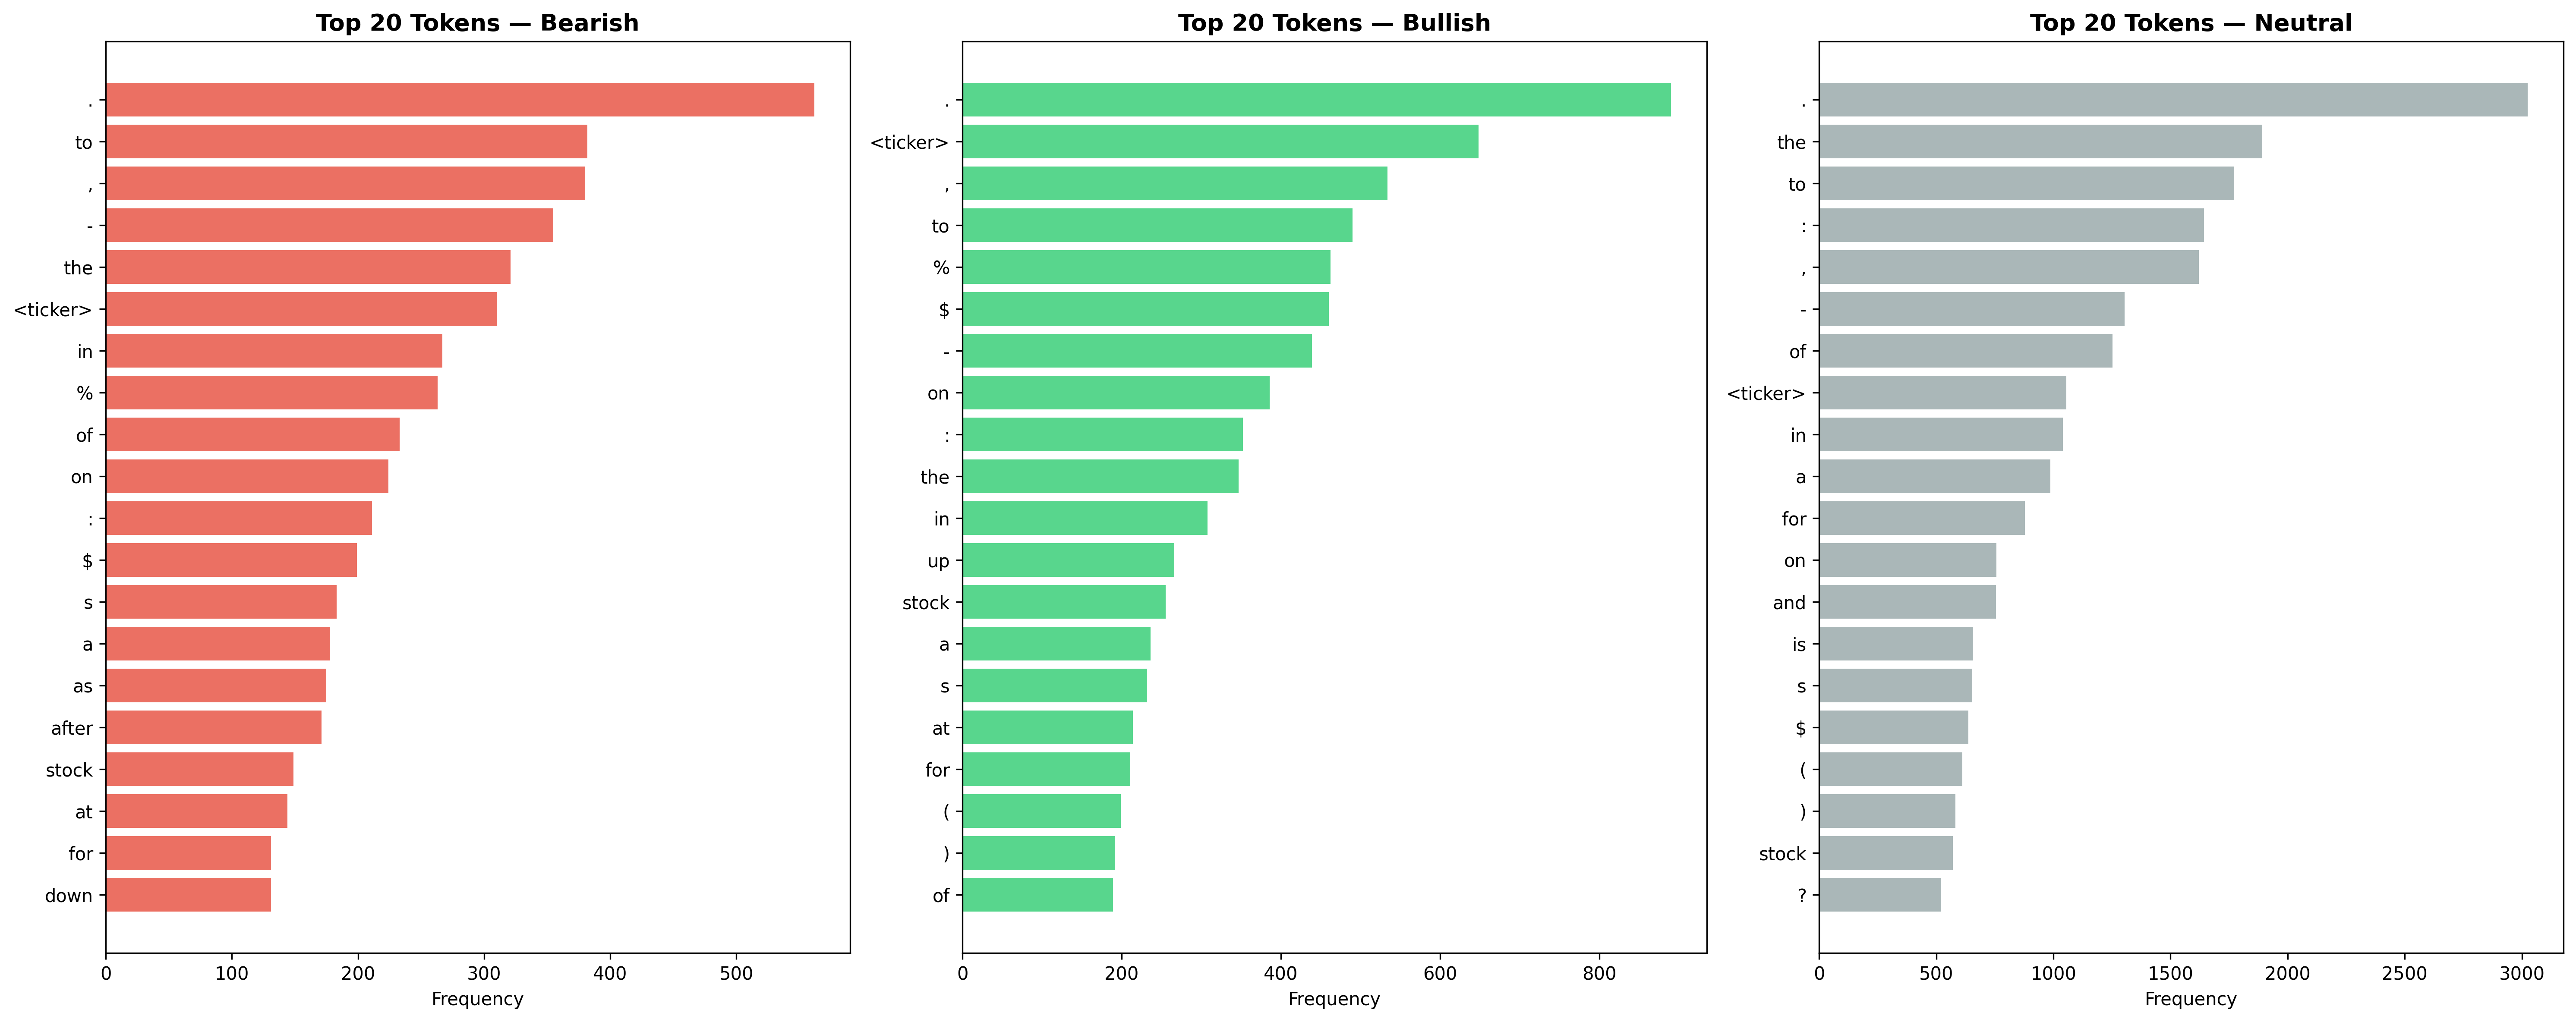
\includegraphics[width=\textwidth]{top_tokens_per_class.png}
    \caption{Top tokens per class.}
\end{subfigure}
\hfill
\begin{subfigure}[t]{0.48\textwidth}
    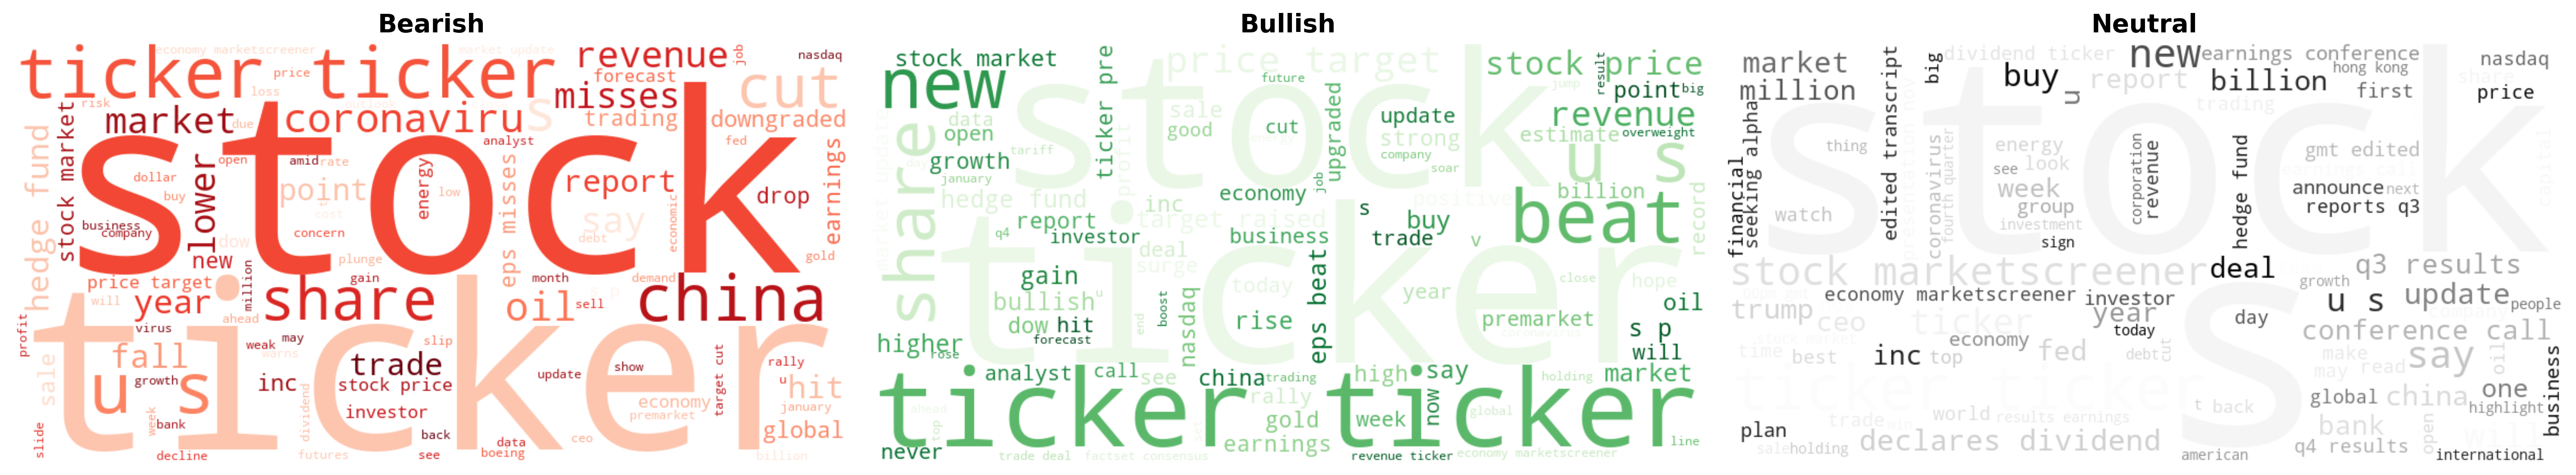
\includegraphics[width=\textwidth]{wordclouds_per_class.png}
    \caption{Word clouds per class.}
\end{subfigure}
\caption{Discriminative vocabulary analysis showing class-specific token patterns.}
\label{fig:vocab}
\end{figure}

\subsection{Data Quality}

\begin{itemize}[nosep]
    \item \textbf{Exact duplicates}: A small number exist ($<$1\%) and are retained to avoid biasing class proportions.
    \item \textbf{Label leakage check}: Words like ``bearish'' and ``bullish'' appear naturally in financial discourse --- they are domain vocabulary, not data leakage.
\end{itemize}

% ============================================================================
% 3. DATA PREPROCESSING
% ============================================================================
\section{Data Preprocessing}

\subsection{Design Philosophy}

We implemented \textbf{composable preprocessing functions} in \texttt{src/preprocessing.py}, allowing us to mix and match cleaning steps into named pipelines. This modular design ensures reproducibility and enables systematic comparison.

\subsection{Preprocessing Functions}

We implement the following cleaning steps, each as a standalone composable function:

\begin{enumerate}[nosep]
    \item \textbf{HTML unescape} --- Decode \texttt{\&amp;}, \texttt{\&lt;}, etc.
    \item \textbf{URL removal} --- Strip \texttt{http://...} and \texttt{www.} links.
    \item \textbf{Mention removal} --- Strip \texttt{@username} handles.
    \item \textbf{Hashtag handling} --- Strip \texttt{\#} but keep the word (e.g., \texttt{\#bullish} $\rightarrow$ \texttt{bullish}).
    \item \textbf{Ticker normalization} --- Replace \texttt{\$AAPL}, \texttt{\$TSLA}, etc.\ with \texttt{<TICKER>}.
    \item \textbf{Number normalization} --- Replace percentages with \texttt{<PCT>}, other numbers with \texttt{<NUM>}.
    \item \textbf{Emoji demojization} --- Convert emojis to text descriptions (e.g., rocket emoji $\rightarrow$ ``rocket''), preserving sentiment signal.
    \item \textbf{Unicode normalization} --- NFKC normalization for consistent character encoding.
    \item \textbf{Lowercasing} --- Standard case folding.
    \item \textbf{Punctuation collapsing} --- \texttt{!!!} $\rightarrow$ \texttt{!}, whitespace normalization.
    \item \textbf{Financial-aware stopword removal} --- We customize the NLTK English stopword list by \textbf{keeping} negations (\texttt{no}, \texttt{not}, \texttt{nor}, \texttt{against}) and directional words (\texttt{up}, \texttt{down}, \texttt{over}, \texttt{under}). These are critical for financial sentiment --- ``not going up'' means the opposite of ``going up''.
    \item \textbf{Lemmatization} (WordNet) and \textbf{Stemming} (Porter) --- Tested as optional operations.
\end{enumerate}

\subsection{Named Pipelines}

\begin{table}[H]
\centering
\caption{Preprocessing pipelines and their target use cases.}
\label{tab:pipelines}
\begin{tabular}{llp{6cm}}
\toprule
\textbf{Pipeline} & \textbf{Steps} & \textbf{Use Case} \\
\midrule
\texttt{pp\_minimal} & 1--10 & BoW, TF-IDF, Word2Vec \\
\texttt{pp\_aggressive} & 1--12 (+ stopwords, lemma) & Tested, dropped \\
\texttt{pp\_transformer} & 1--7, 10 (no lowercase) & Transformer inputs \\
\bottomrule
\end{tabular}
\end{table}

\subsection{Pipeline Comparison}

We benchmarked \texttt{pp\_minimal} vs.\ \texttt{pp\_aggressive} using the same classifier (LogReg + TF-IDF) to isolate the preprocessing effect:

\begin{table}[H]
\centering
\caption{Preprocessing pipeline comparison (LogReg + TF-IDF baseline).}
\begin{tabular}{lr}
\toprule
\textbf{Pipeline} & \textbf{Macro-F1} \\
\midrule
\texttt{pp\_minimal} & \textbf{0.736} \\
\texttt{pp\_aggressive} (lemma) & 0.718 \\
\texttt{pp\_aggressive} (stem) & 0.709 \\
\bottomrule
\end{tabular}
\end{table}

\textbf{Result}: \texttt{pp\_minimal} consistently outperforms \texttt{pp\_aggressive}. The aggressive pipeline destroys discriminative signal by:
\begin{itemize}[nosep]
    \item Removing stopwords that include negations like ``not'' that flip sentiment.
    \item Lemmatizing temporal distinctions (``falling'' $\rightarrow$ ``fall'') that carry urgency information.
    \item Normalizing numbers removes specific price/percentage values providing context.
\end{itemize}

\textbf{Decision}: \texttt{pp\_minimal} is used for all traditional ML experiments. \texttt{pp\_transformer} is used for Transformer feature extraction, where pretrained tokenizers handle subword splitting.

% ============================================================================
% 4. FEATURE ENGINEERING
% ============================================================================
\section{Feature Engineering}

We implement and compare \textbf{eight feature extraction methods} across three families.

\subsection{Bag-of-Words Features (Mandatory)}

\textbf{CountVectorizer (BoW)}: Unigram counts with a vocabulary cap of 10,000 features. Serves as the simplest baseline.

\textbf{TF-IDF}: Our optimized configuration uses bigrams (\texttt{ngram\_range=(1,2)}) to capture phrases like ``going up'' and ``sell off'', sublinear TF scaling to dampen very frequent terms, and a maximum of 20,000 features with \texttt{min\_df=2} and \texttt{max\_df=0.95}.

TF-IDF with bigrams outperforms BoW by 1--3 percentage points across all classifiers, confirming that word order carries sentiment signal even in a bag-of-words framework.

\begin{figure}[H]
\centering
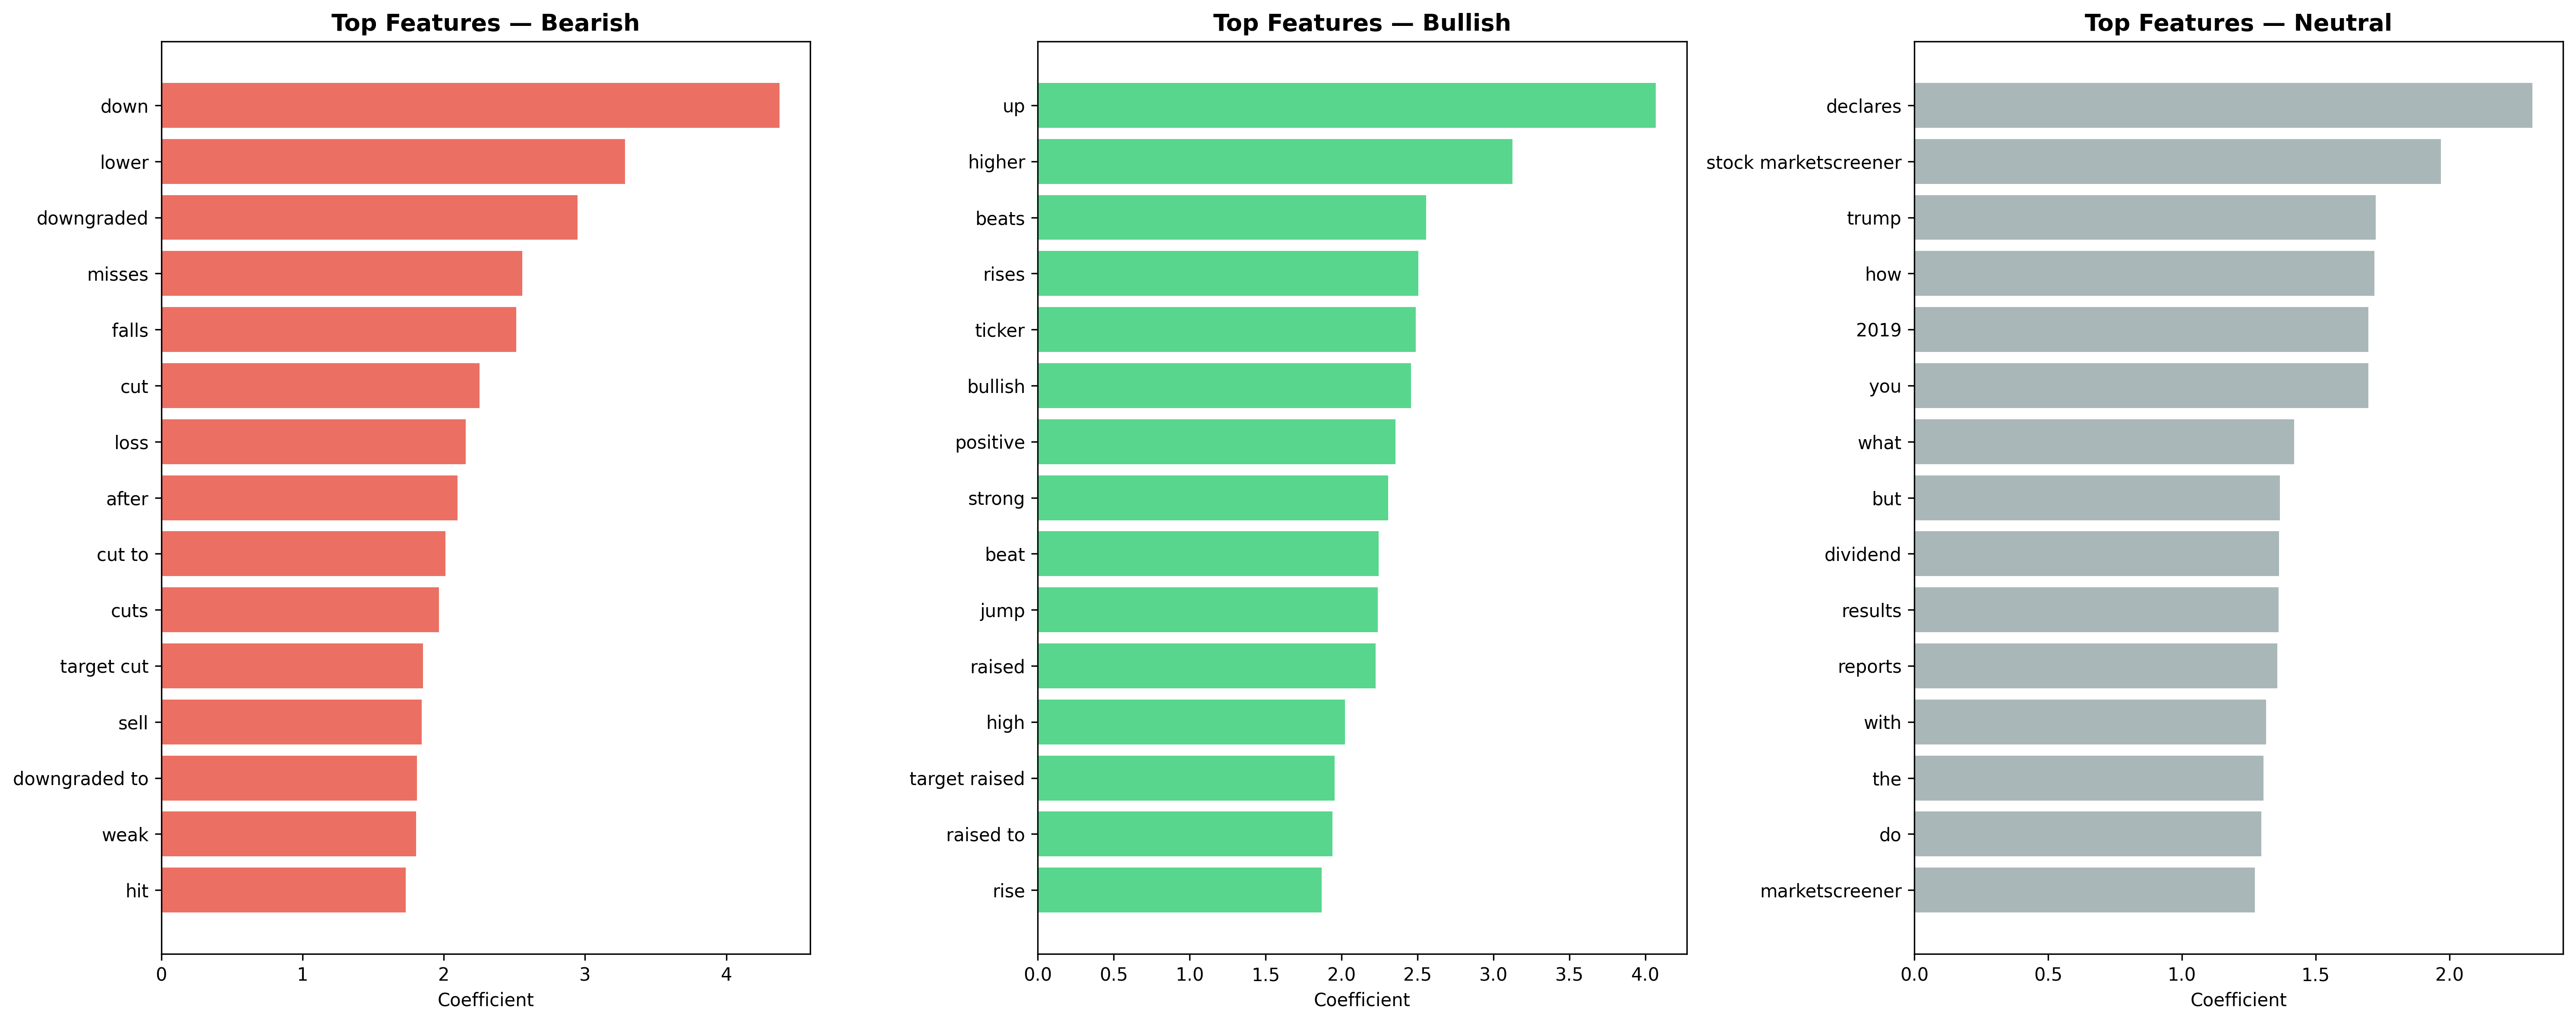
\includegraphics[width=0.85\textwidth]{top_tfidf_features.png}
\caption{Top TF-IDF features per class, extracted from Logistic Regression coefficients.}
\label{fig:tfidf_features}
\end{figure}

\subsection{Word Embeddings (Mandatory)}

\textbf{Custom Word2Vec}: Skip-gram model trained on the financial tweet corpus (100 dimensions, window=5, min\_count=2, 20 epochs). Document representations are computed via mean pooling of token embeddings.

\textbf{Pretrained GloVe Twitter 100d}: Pretrained on 2 billion tweets, providing general Twitter vocabulary coverage but lacking financial domain specificity.

\textbf{TF-IDF-Weighted Pooling}: Weights each token's embedding by its TF-IDF score before averaging, giving more importance to rare, discriminative words.

\textbf{Results}: All Word2Vec variants perform significantly worse than BoW/TF-IDF (macro-F1: 0.59--0.66 vs.\ 0.72--0.74). The primary reason is that \textbf{mean pooling loses word order information}, which is critical for sentiment. ``Stock going up'' and ``stock going down'' produce similar mean vectors despite opposite sentiments.

\subsection{Transformer Encoders (Mandatory + Extra Work)}

\textbf{Strategy}: We use pretrained Transformer encoders as \textbf{frozen feature extractors}. For each tweet, we tokenize with the model's pretrained tokenizer, pass through the frozen encoder, mean-pool the last hidden states (768-dimensional) with attention mask weighting, and use the resulting vector as input to a downstream sklearn classifier. Embeddings are cached as \texttt{.npy} files, making this CPU-feasible.

\begin{table}[H]
\centering
\caption{Transformer encoders evaluated as frozen feature extractors.}
\label{tab:transformers}
\begin{tabular}{llll}
\toprule
\textbf{Encoder} & \textbf{Domain} & \textbf{Params} & \textbf{Status} \\
\midrule
DistilBERT & General & 66M & Mandatory \\
FinBERT & Finance (SEC filings) & 110M & Extra work \\
Twitter-RoBERTa & Twitter + sentiment & 125M & Extra work \\
\bottomrule
\end{tabular}
\end{table}

\textbf{Key finding}: Domain alignment is more important than model size. DistilBERT (general-purpose, 66M params) underperforms TF-IDF, while Twitter-RoBERTa (tweet-domain, sentiment-tuned, 125M params) achieves the best results overall. FinBERT falls between --- it understands financial language but was trained on formal SEC filings, not informal tweets.

% ============================================================================
% 5. CLASSIFICATION MODELS
% ============================================================================
\section{Classification Models}

\subsection{Classifiers Evaluated}

\begin{table}[H]
\centering
\caption{Classifiers and their key hyperparameters.}
\label{tab:classifiers}
\small
\begin{tabular}{lp{5cm}p{4.5cm}}
\toprule
\textbf{Classifier} & \textbf{Key Hyperparameters} & \textbf{Rationale} \\
\midrule
Logistic Regression & balanced, C=1.0, multinomial & Interpretable baseline \\
LinearSVC & balanced, C=1.0 & Maximum-margin, sparse data \\
XGBoost & 300 trees, depth=6, softprob & Non-linear boundaries \\
Random Forest & 300 trees, balanced & Ensemble baseline \\
\bottomrule
\end{tabular}
\normalsize
\end{table}

All classifiers use class weighting to handle class imbalance by upweighting minority classes.

\subsection{Evaluation Protocol}

\begin{itemize}[nosep]
    \item \textbf{5-fold Stratified K-Fold Cross-Validation} preserving class proportions in each fold
    \item \textbf{Primary metric}: Macro-F1 (equally weights all three classes)
    \item \textbf{Reproducibility}: \texttt{random\_state=42} for all stochastic operations
\end{itemize}

% ============================================================================
% 6. RESULTS AND ANALYSIS
% ============================================================================
\section{Results and Analysis}

\subsection{Full Results Matrix}

\begin{table}[H]
\centering
\caption{Macro-F1 scores (mean $\pm$ std) across all 32 feature $\times$ classifier combinations, evaluated via 5-fold stratified cross-validation. \textbf{Bold} marks the best score per row; \underline{underline} marks the overall best. *Extra work.}
\label{tab:results}
\small
\begin{tabular}{l|cccc}
\toprule
\textbf{Features} & \textbf{LogReg} & \textbf{SVM} & \textbf{XGBoost} & \textbf{RandForest} \\
\midrule
BoW & \textbf{.720$\pm$.011} & .708$\pm$.010 & .691$\pm$.013 & .664$\pm$.012 \\
TF-IDF & .736$\pm$.006 & \textbf{.740$\pm$.013} & .670$\pm$.011 & .654$\pm$.014 \\
W2V-mean & .600$\pm$.013 & .603$\pm$.012 & \textbf{.650$\pm$.006} & .595$\pm$.011 \\
W2V-tfidf & .595$\pm$.013 & .610$\pm$.015 & \textbf{.658$\pm$.016} & .611$\pm$.011 \\
GloVe-mean & .599$\pm$.017 & .617$\pm$.014 & \textbf{.636$\pm$.009} & .494$\pm$.004 \\
DistilBERT & .702$\pm$.009 & \textbf{.705$\pm$.008} & .674$\pm$.012 & .517$\pm$.007 \\
FinBERT* & .736$\pm$.007 & .751$\pm$.009 & \textbf{.779$\pm$.003} & .734$\pm$.002 \\
Twitter-RoBERTa* & .755$\pm$.011 & .764$\pm$.008 & \underline{\textbf{.794$\pm$.006}} & .742$\pm$.008 \\
\bottomrule
\end{tabular}
\end{table}

\subsection{Key Findings}

\textbf{Feature hierarchy} (most to least effective):
\begin{enumerate}[nosep]
    \item \textbf{Twitter-RoBERTa} (best: 0.794) --- Pretrained on 58M tweets with sentiment labels; perfect domain alignment for our task.
    \item \textbf{FinBERT} (best: 0.779) --- Financial domain knowledge helps, but trained on formal SEC filings rather than informal tweets.
    \item \textbf{TF-IDF} (best: 0.740) --- Surprisingly competitive. Bigram TF-IDF captures local word order patterns that discriminate sentiment.
    \item \textbf{BoW} (best: 0.720) --- Solid baseline, but loses the bigram advantage.
    \item \textbf{DistilBERT} (best: 0.705) --- General-purpose encoder \textit{underperforms} TF-IDF. Domain alignment matters more than model sophistication.
    \item \textbf{Word2Vec variants} (best: 0.658) --- Mean pooling destroys word order, critical for sentiment.
\end{enumerate}

\textbf{Classifier patterns}:
\begin{itemize}[nosep]
    \item \textbf{XGBoost excels with dense features} (Transformer embeddings): It can learn non-linear decision boundaries in the 768-dimensional embedding space. However, it struggles with sparse features (BoW/TF-IDF) where it must split on individual token presence/absence.
    \item \textbf{Linear models (LogReg, SVM) excel with sparse features}: Regularization handles high-dimensional sparse inputs well. The linear decision boundary is sufficient when features are already semantically meaningful.
    \item \textbf{Random Forest consistently underperforms}: It struggles with both sparse high-dimensional features and dense features (less effective than boosting).
\end{itemize}

\textbf{Stability}: All standard deviations are below 0.017. The best model has one of the lowest ($\pm$0.006), indicating consistent performance across data splits.

\subsection{Per-Class Analysis}

\begin{figure}[H]
\centering
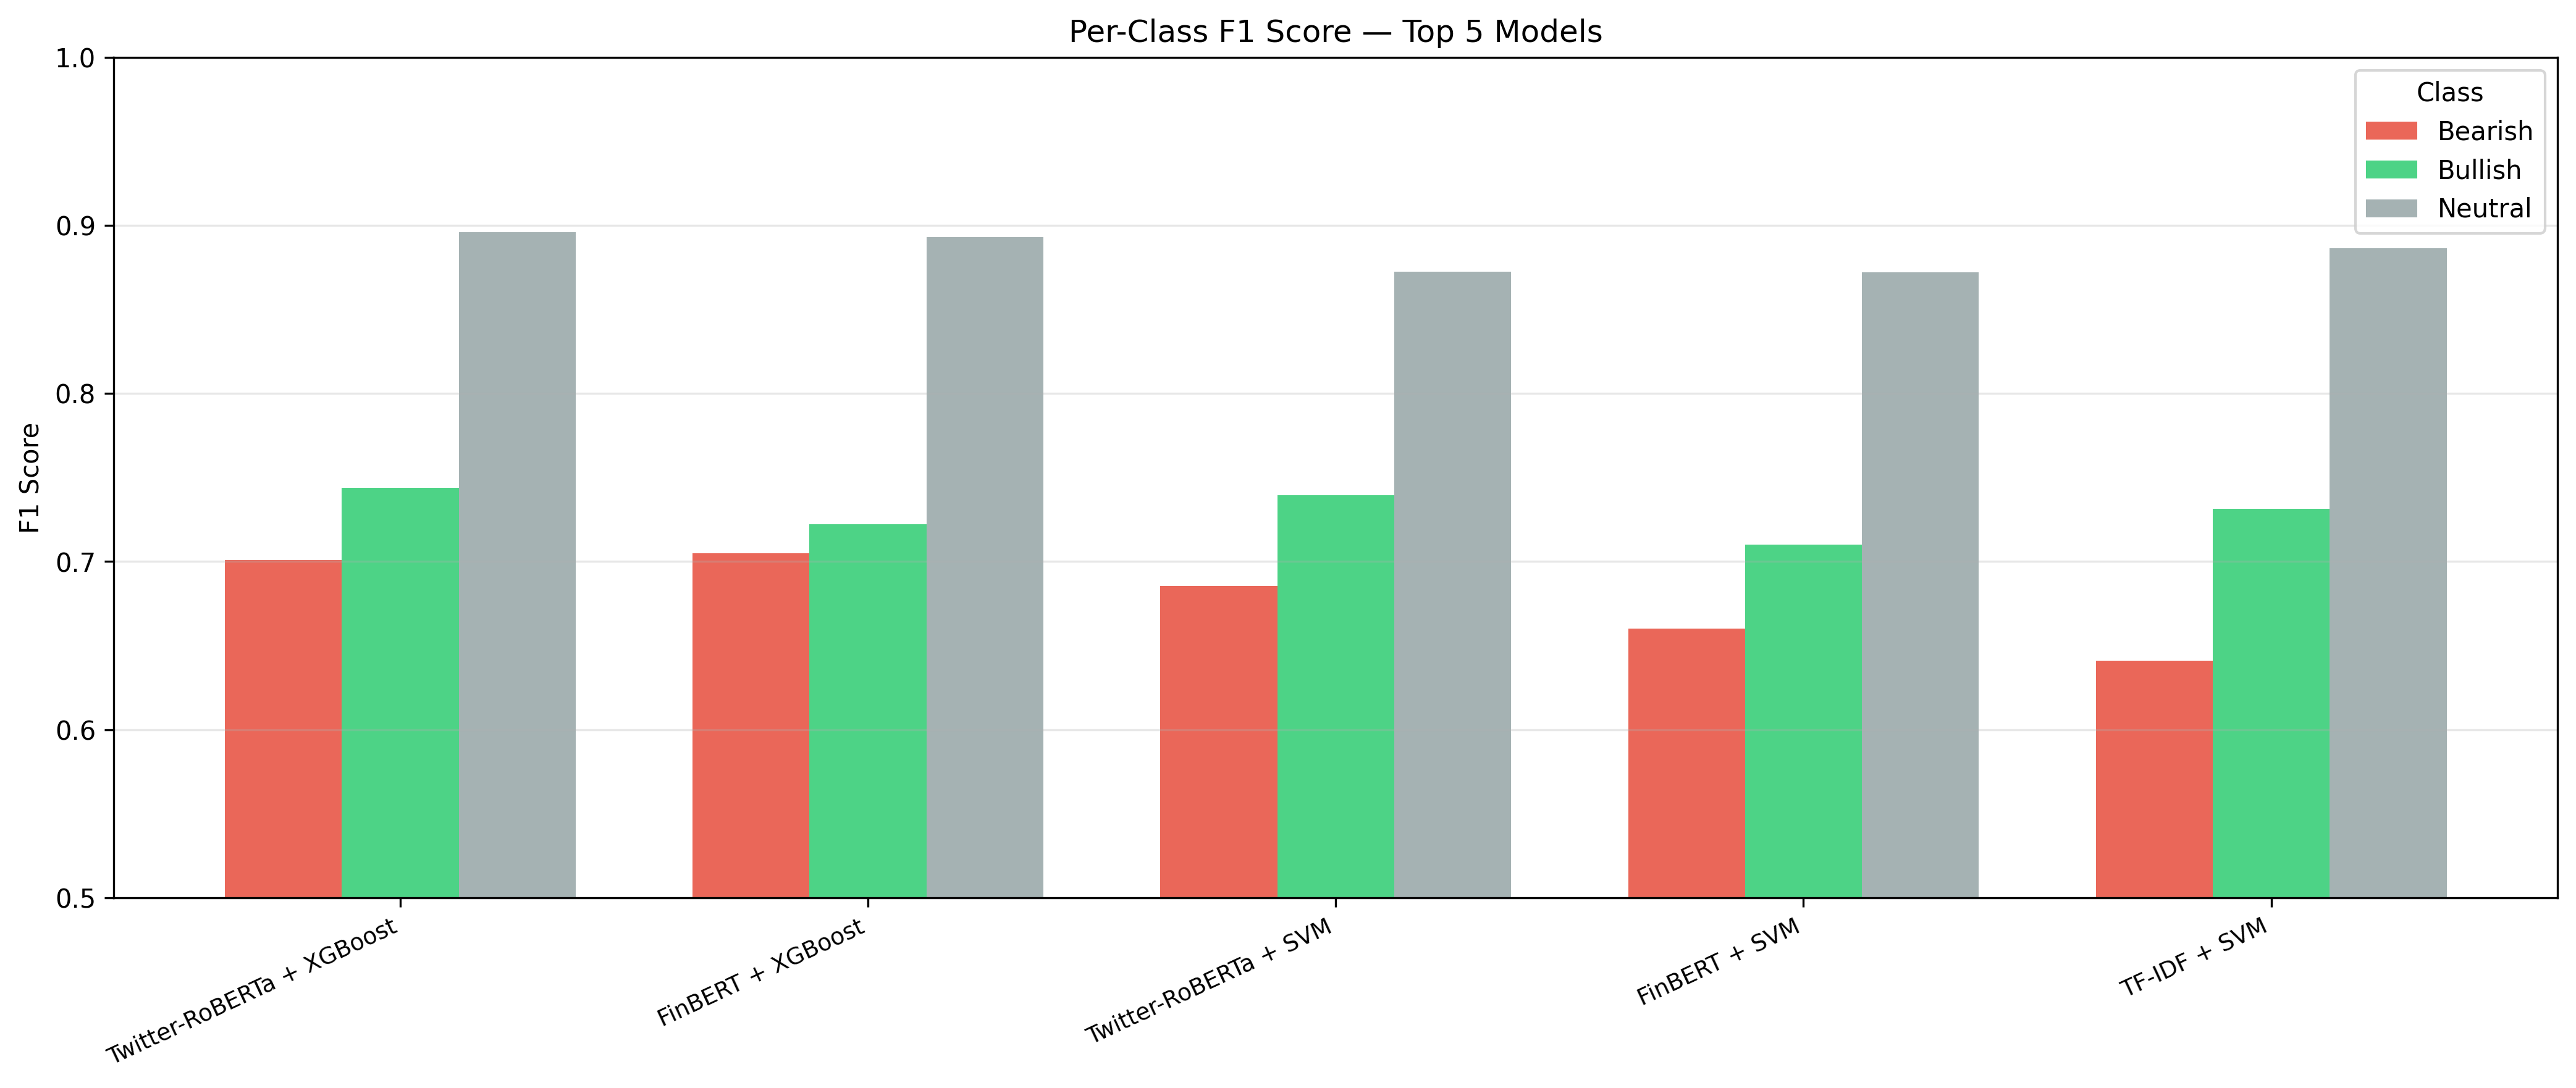
\includegraphics[width=0.88\textwidth]{per_class_f1_top5.png}
\caption{Per-class F1 scores for the top~5 model configurations, showing that Bearish and Bullish are consistently harder to classify than Neutral.}
\label{fig:per_class}
\end{figure}

Analysis of per-class F1 scores reveals:
\begin{itemize}[nosep]
    \item \textbf{Neutral} is consistently the easiest class (F1 $>$ 0.87) due to large support and distinctive factual vocabulary.
    \item \textbf{Bearish} and \textbf{Bullish} are harder (F1: 0.65--0.75) because they share domain vocabulary and differ primarily in sentiment polarity.
    \item \textbf{Bearish} is slightly harder than Bullish --- bearish tweets sometimes use hedging language (``might drop'', ``could fall'') that resembles neutral commentary.
\end{itemize}

\subsection{Error Analysis}

Examining misclassified tweets from the best model reveals common failure patterns:

\begin{enumerate}[nosep]
    \item \textbf{Neutral $\leftrightarrow$ Bearish confusion}: Tweets reporting negative news factually (e.g., ``Stock down 5\% after earnings miss'') are genuinely ambiguous --- the factual reporting is Neutral but the content is inherently negative.
    \item \textbf{Neutral $\leftrightarrow$ Bullish confusion}: Similarly, factual reports of positive events blur the line between informational and positive sentiment.
    \item \textbf{Bearish $\leftrightarrow$ Bullish confusion} (rarest): Occurs primarily with sarcasm or contrarian positions (e.g., ``Great, another day of losses'').
\end{enumerate}

These patterns suggest that the primary challenge is the \textbf{fundamental ambiguity between factual reporting and sentiment expression} in financial discourse.

\begin{figure}[H]
\centering
\begin{subfigure}[t]{0.48\textwidth}
    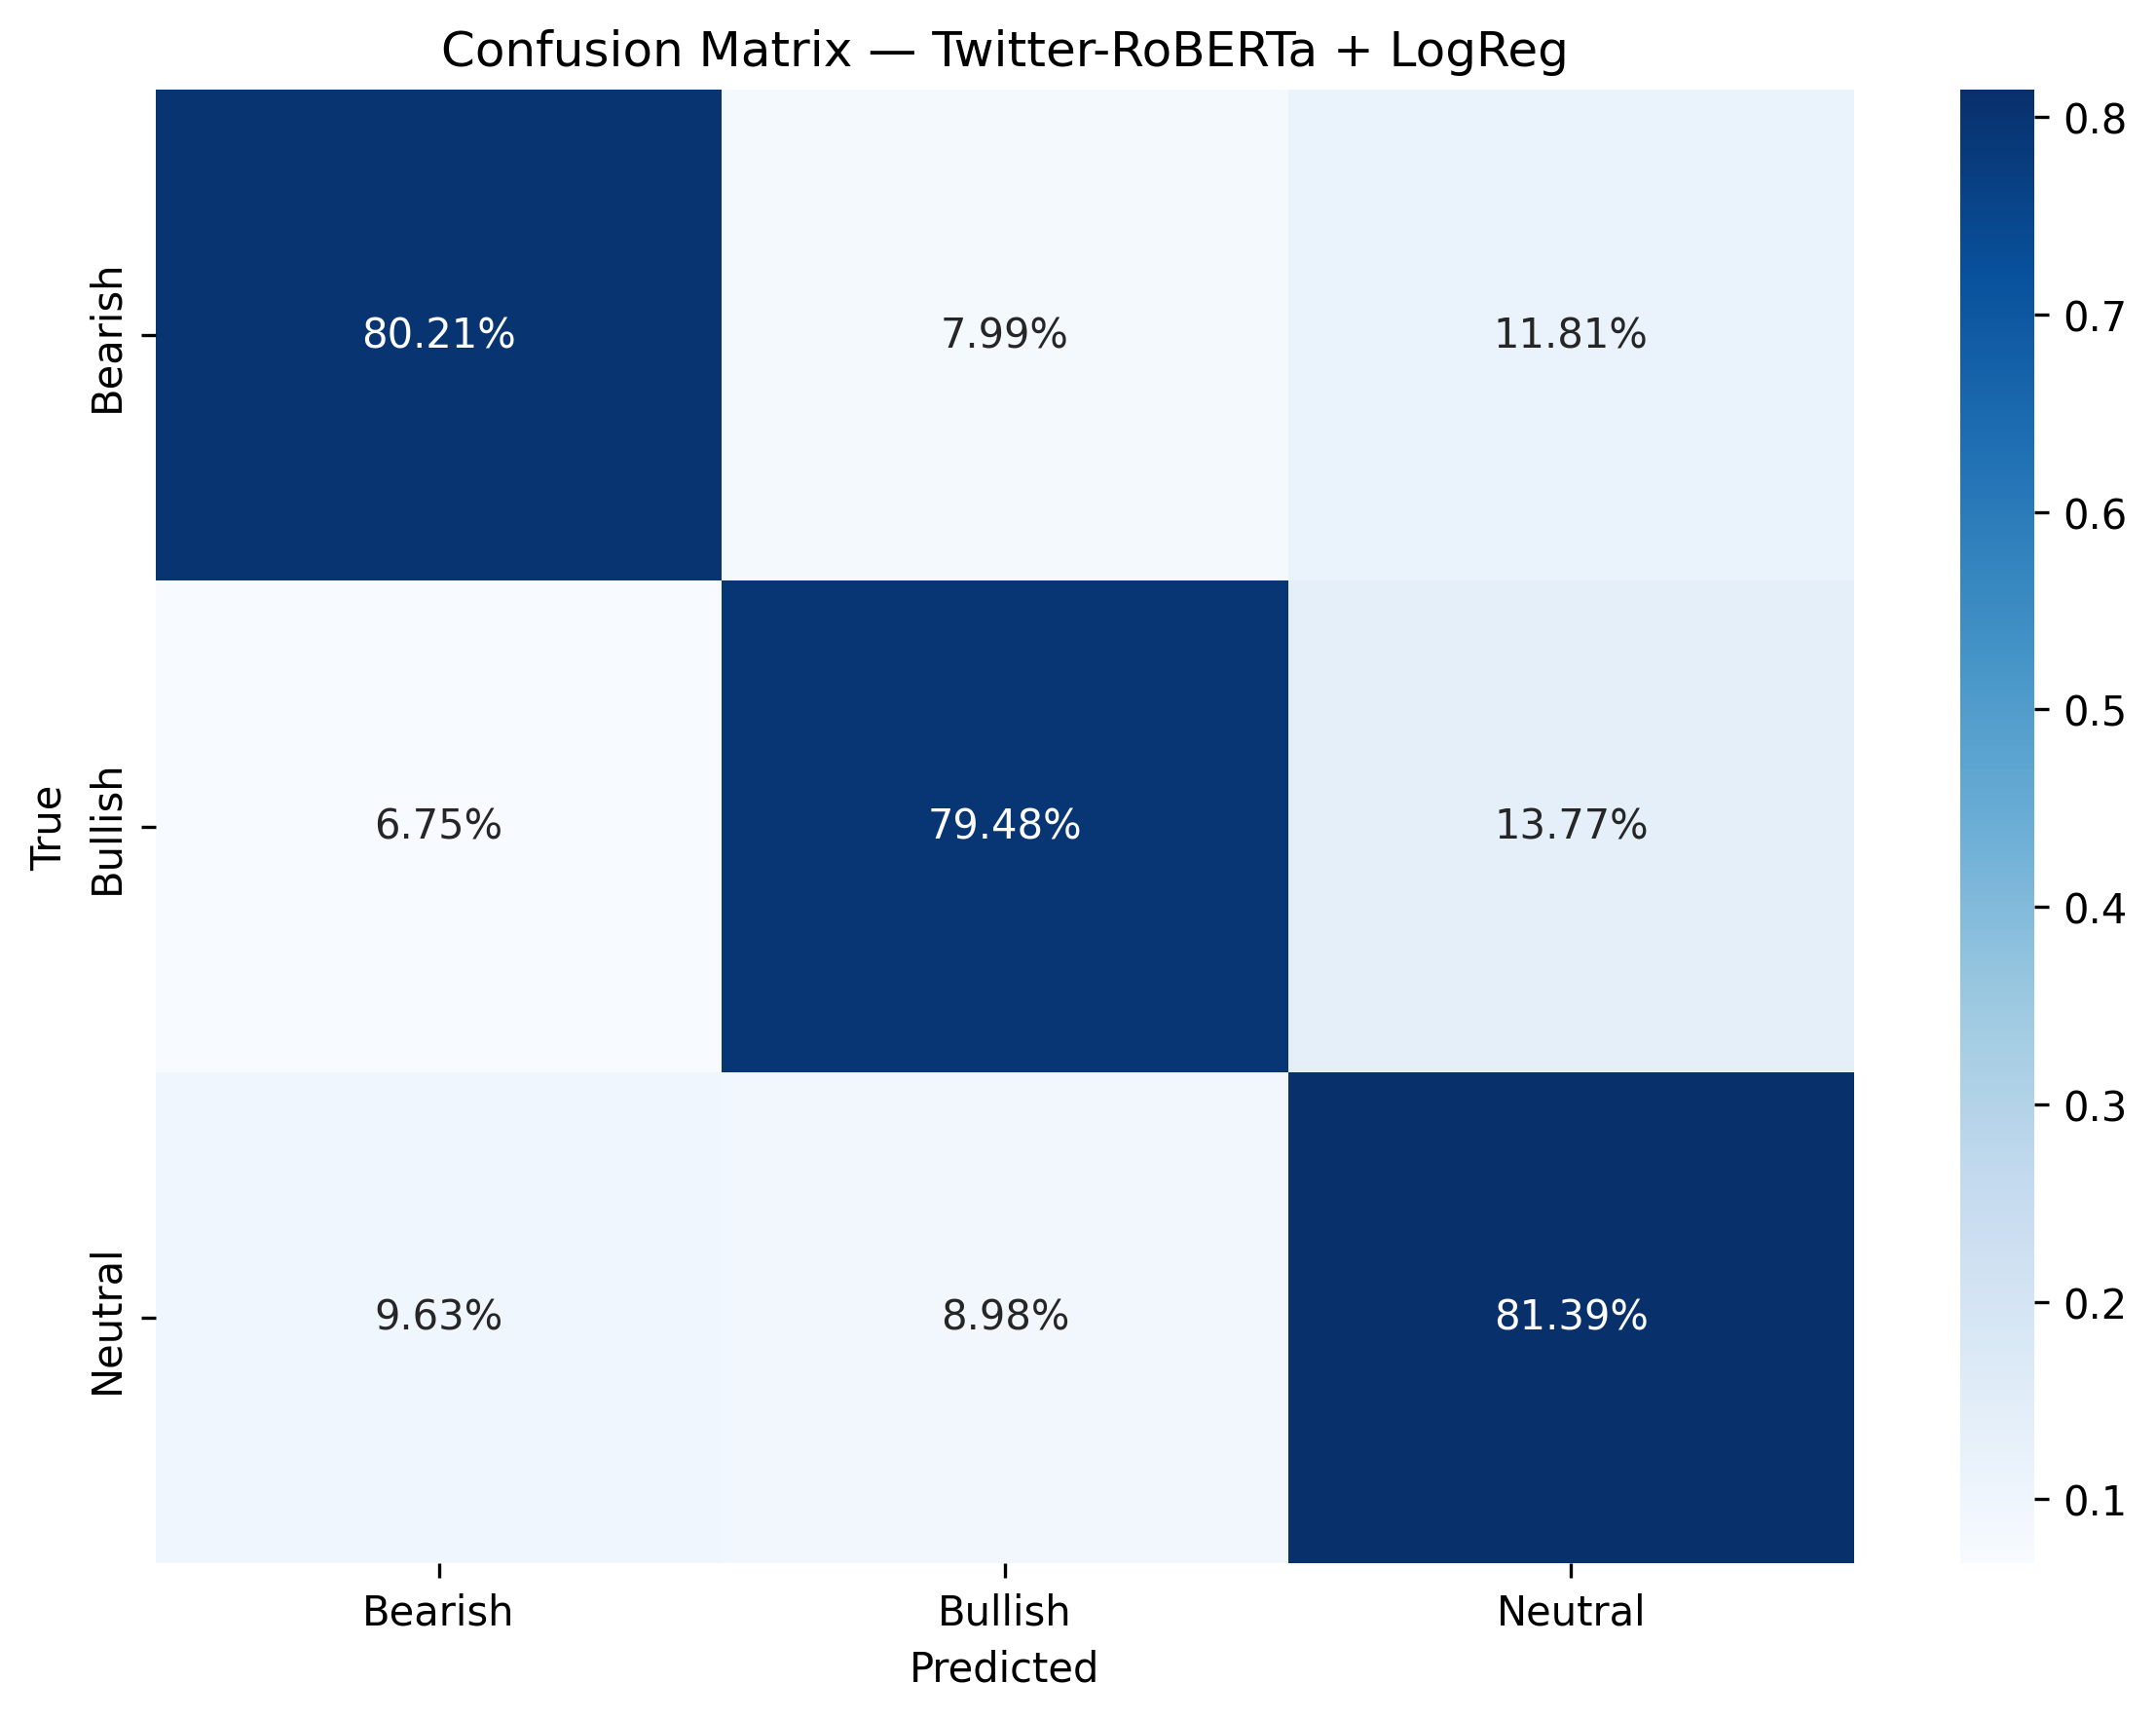
\includegraphics[width=\textwidth]{cm_twitter_roberta.png}
    \caption{Twitter-RoBERTa + XGBoost (best).}
\end{subfigure}
\hfill
\begin{subfigure}[t]{0.48\textwidth}
    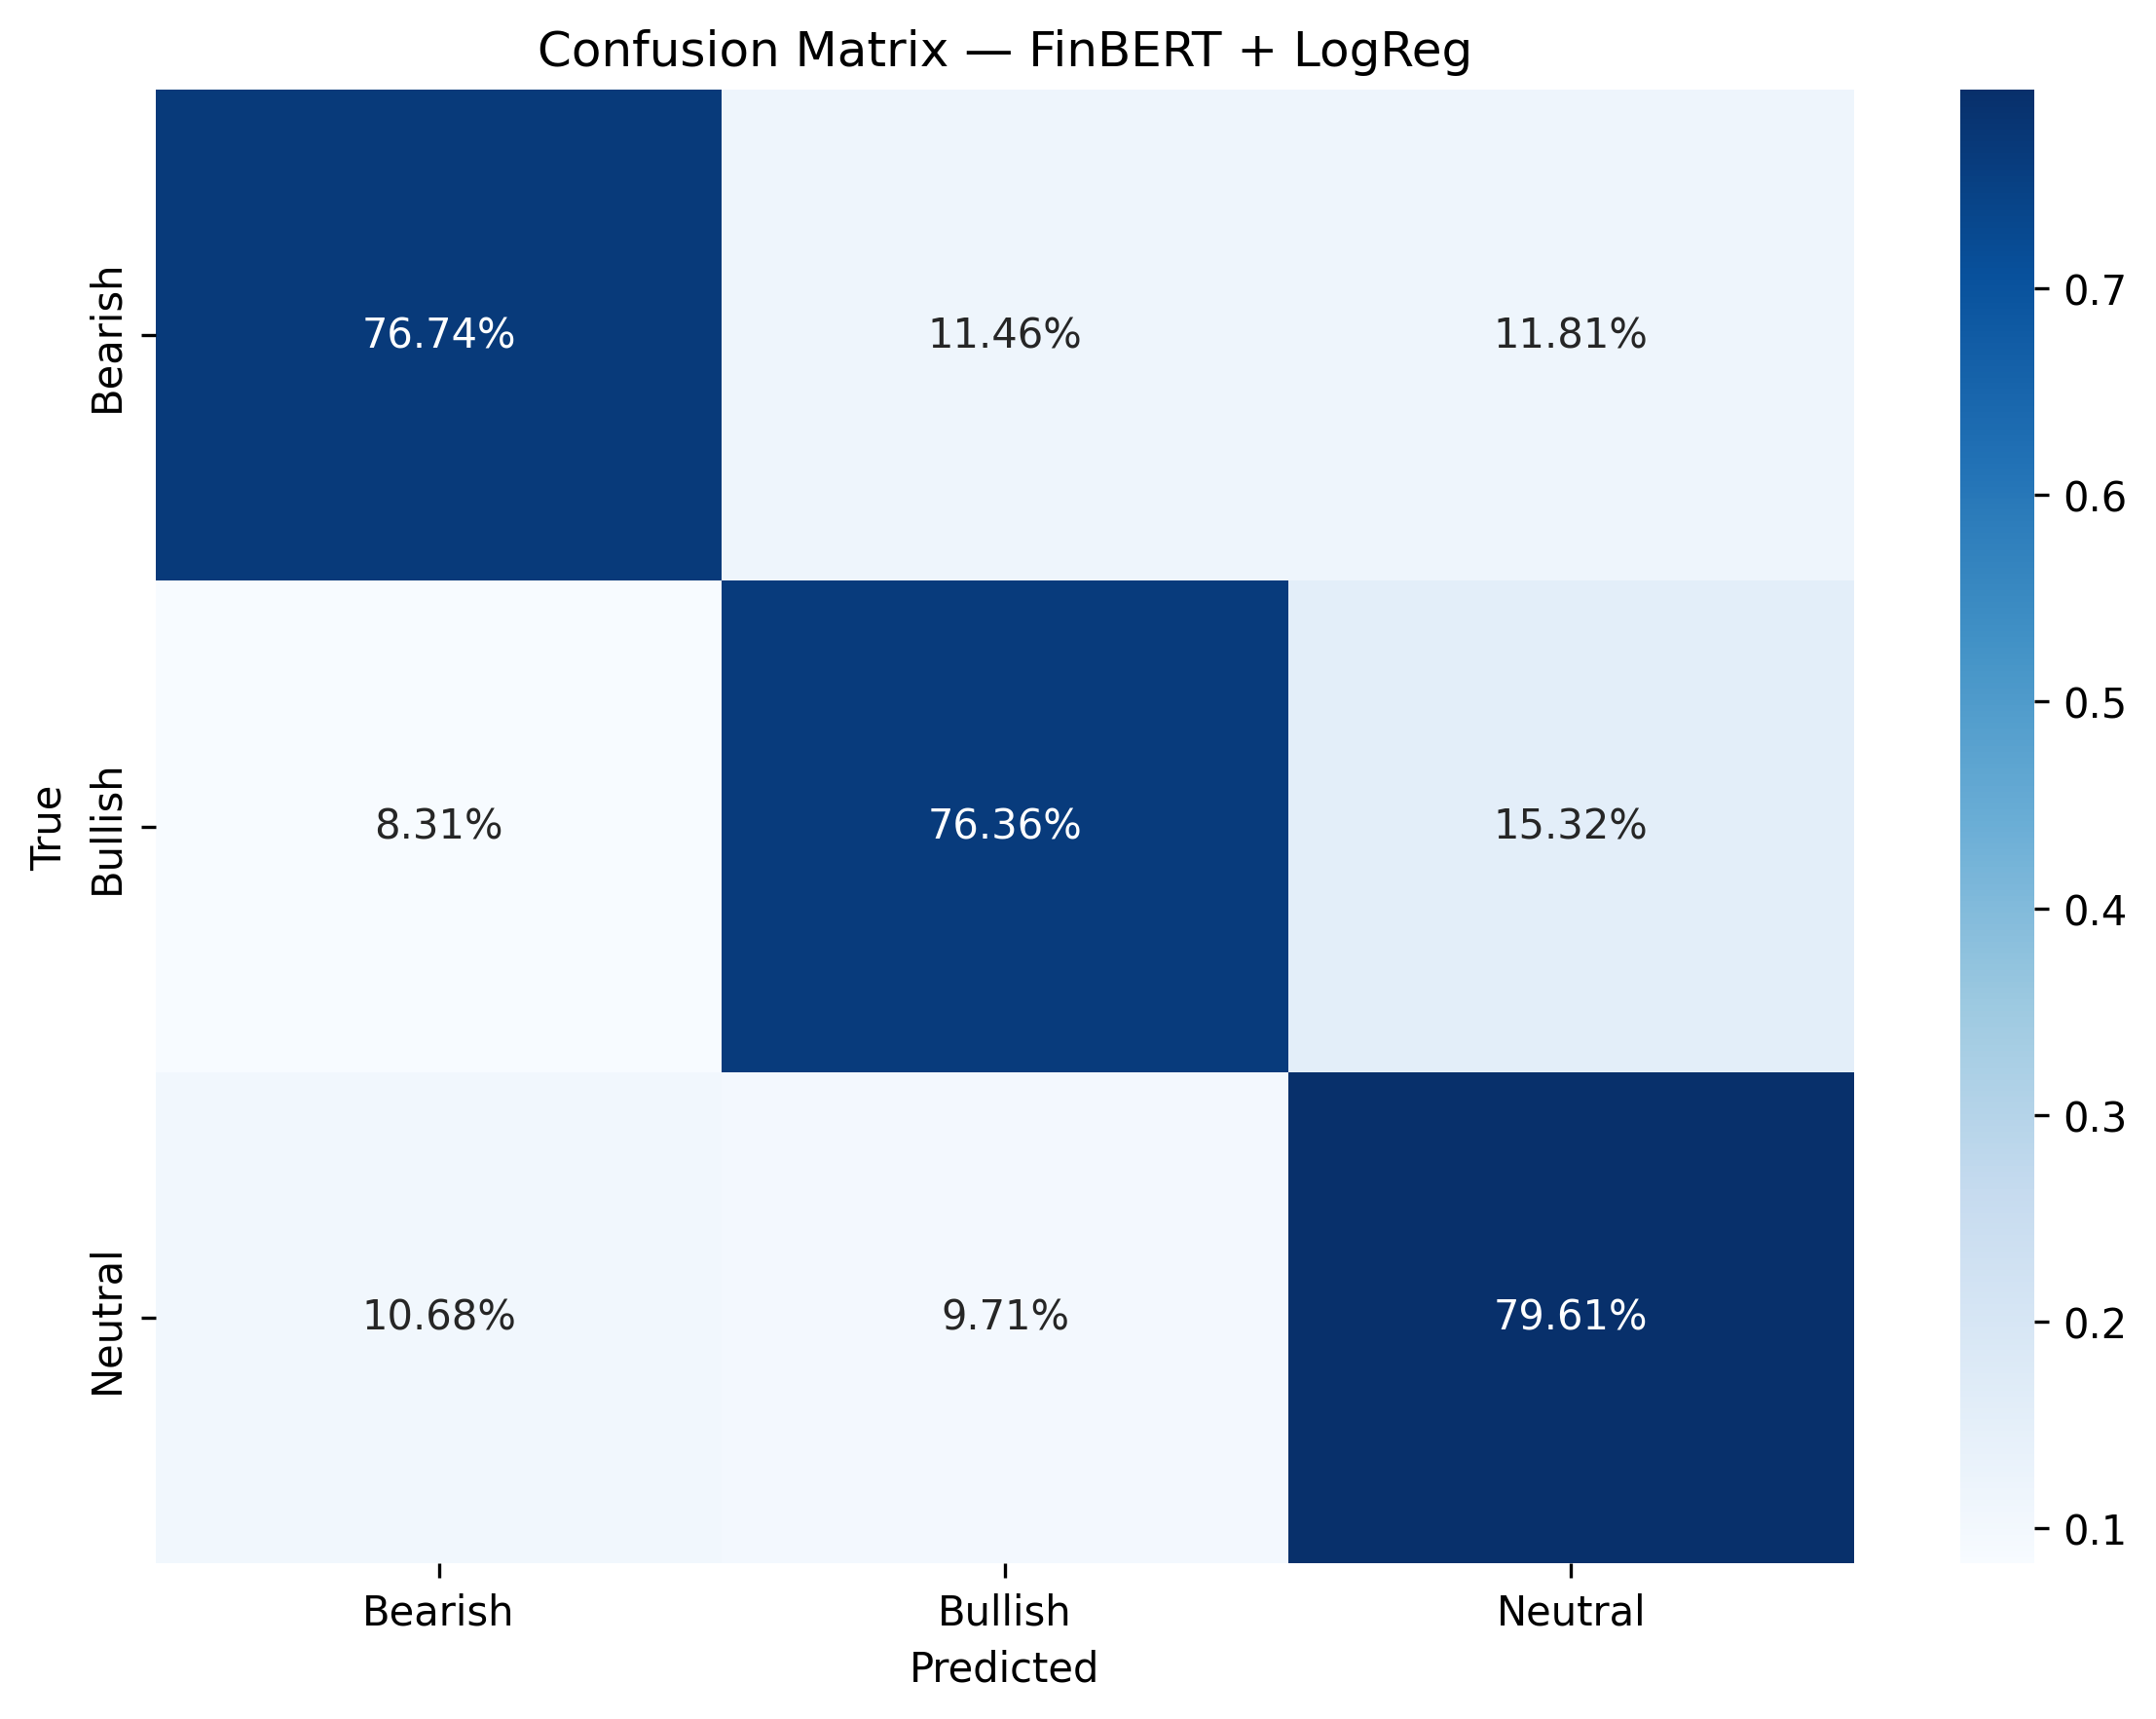
\includegraphics[width=\textwidth]{cm_finbert.png}
    \caption{FinBERT + XGBoost.}
\end{subfigure}
\\[8pt]
\begin{subfigure}[t]{0.48\textwidth}
    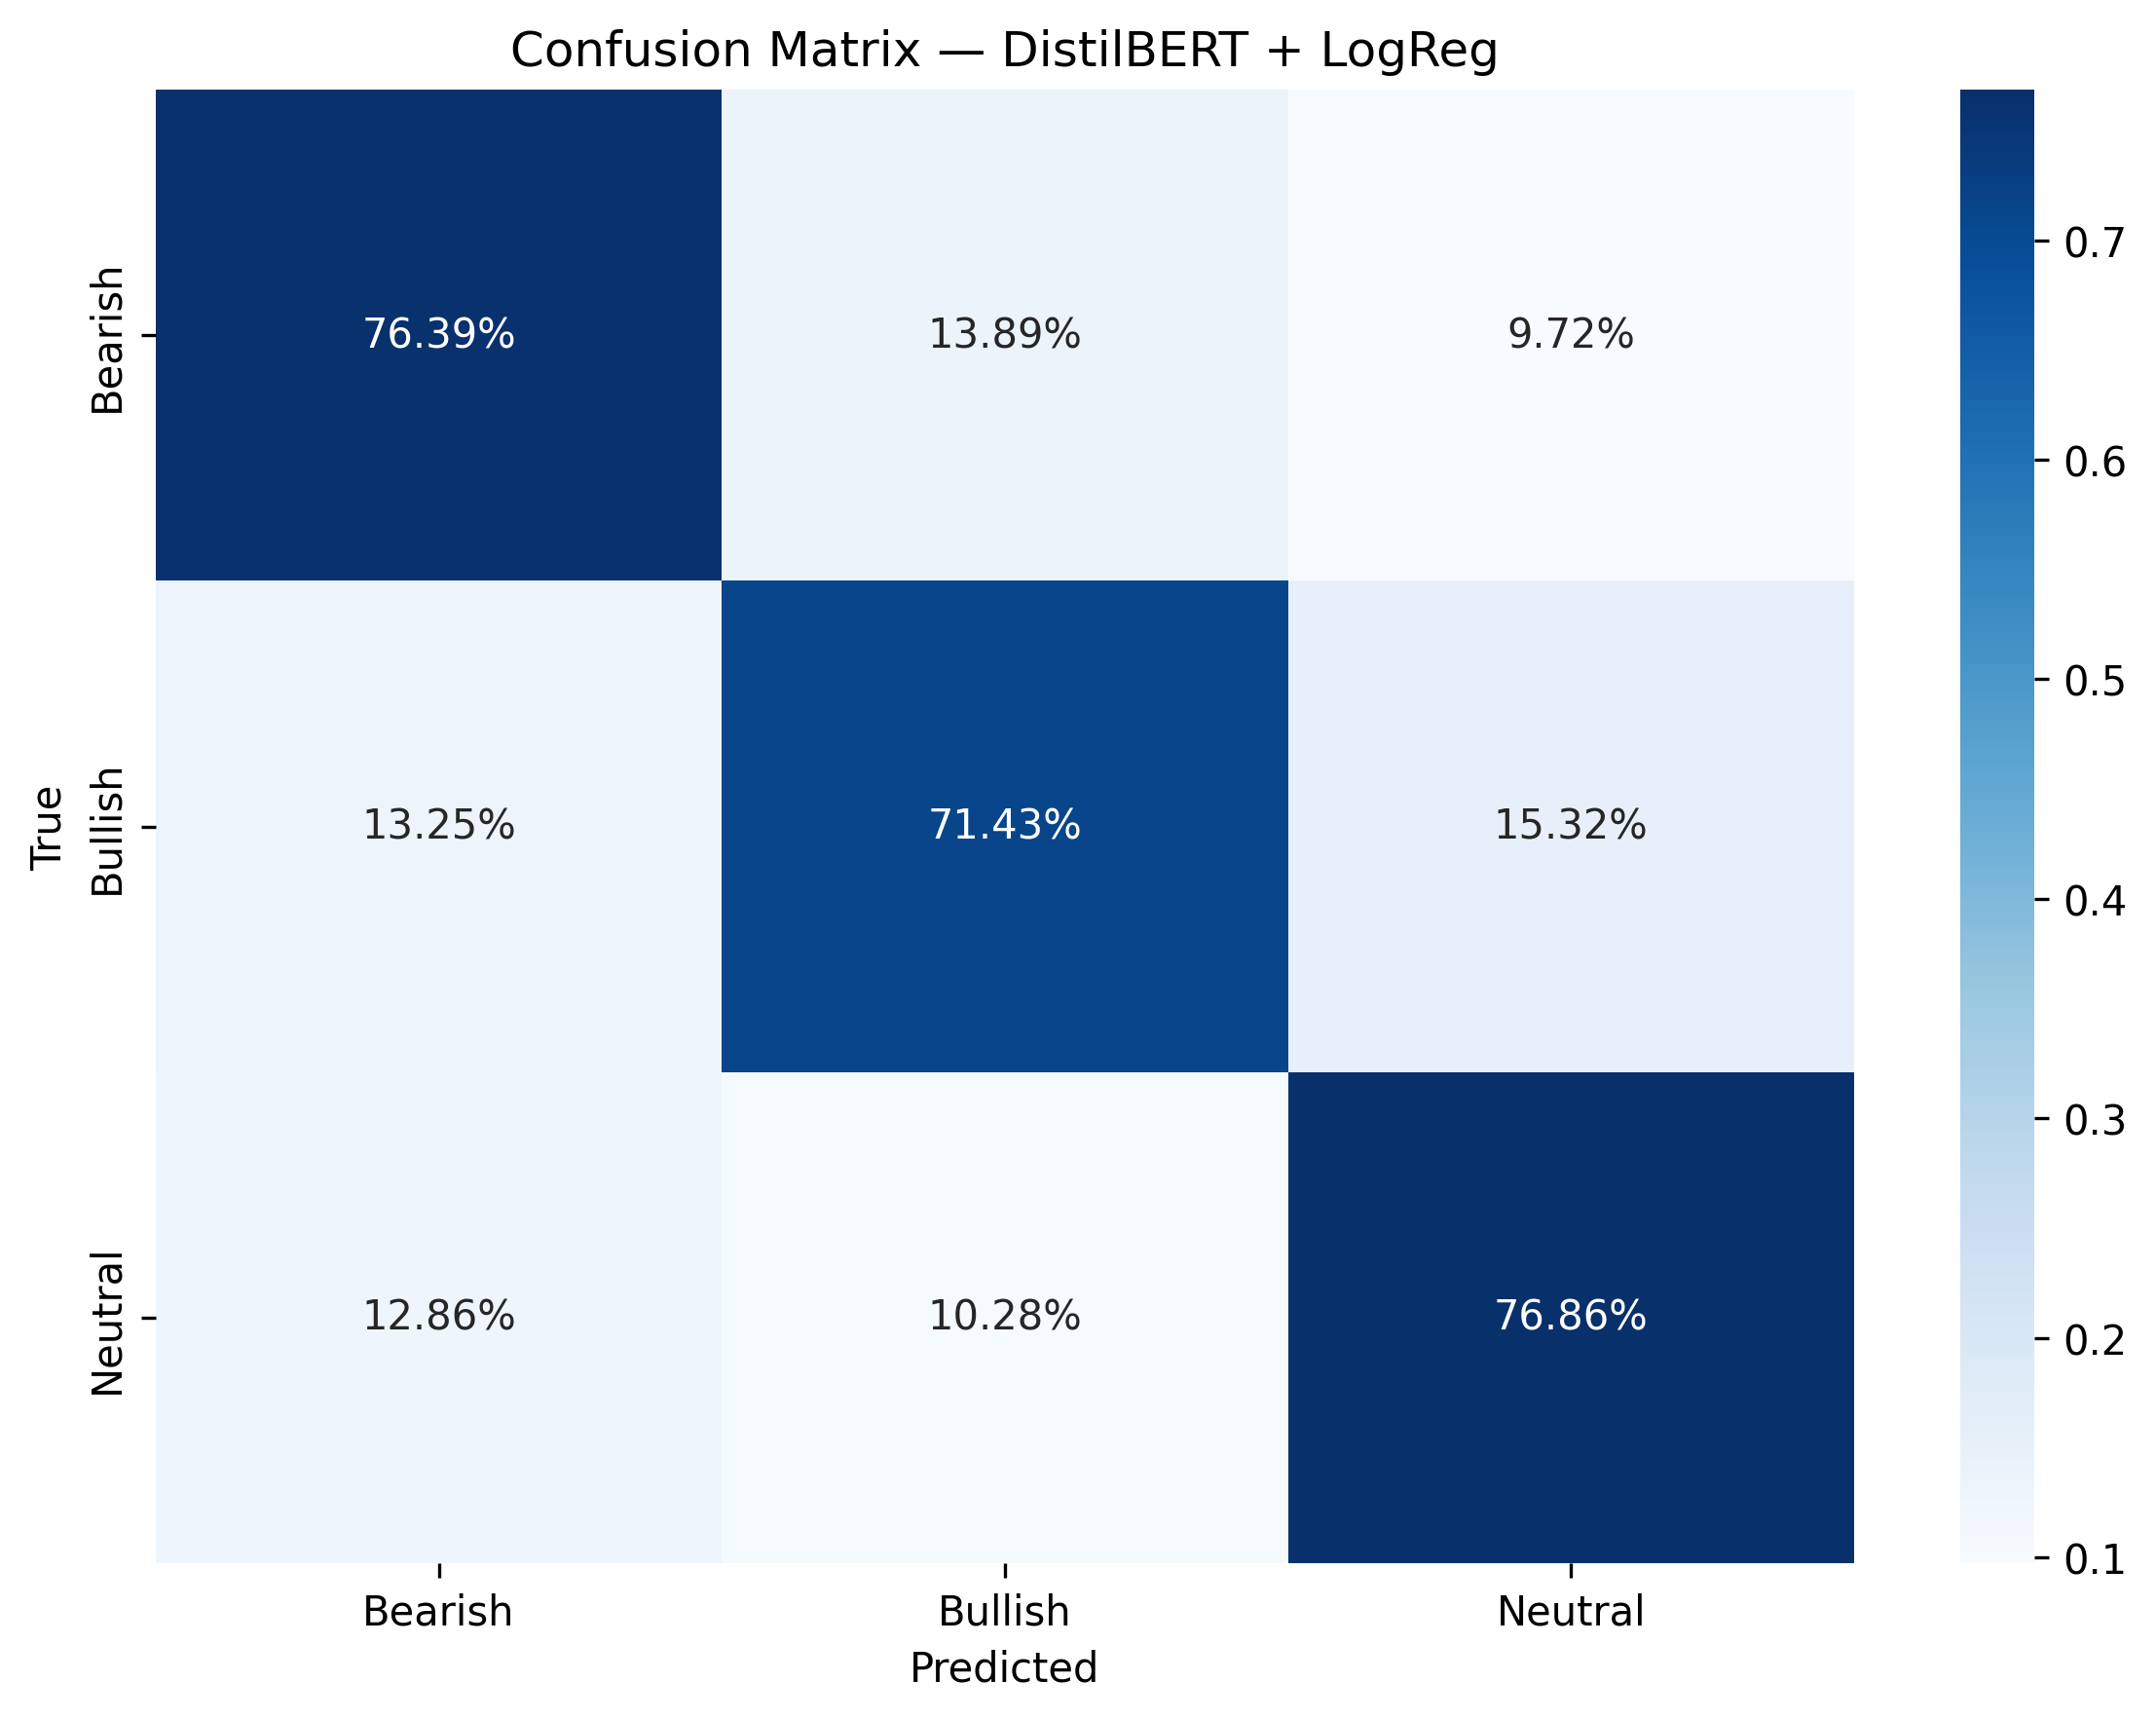
\includegraphics[width=\textwidth]{cm_distilbert.png}
    \caption{DistilBERT + SVM.}
\end{subfigure}
\hfill
\begin{subfigure}[t]{0.48\textwidth}
    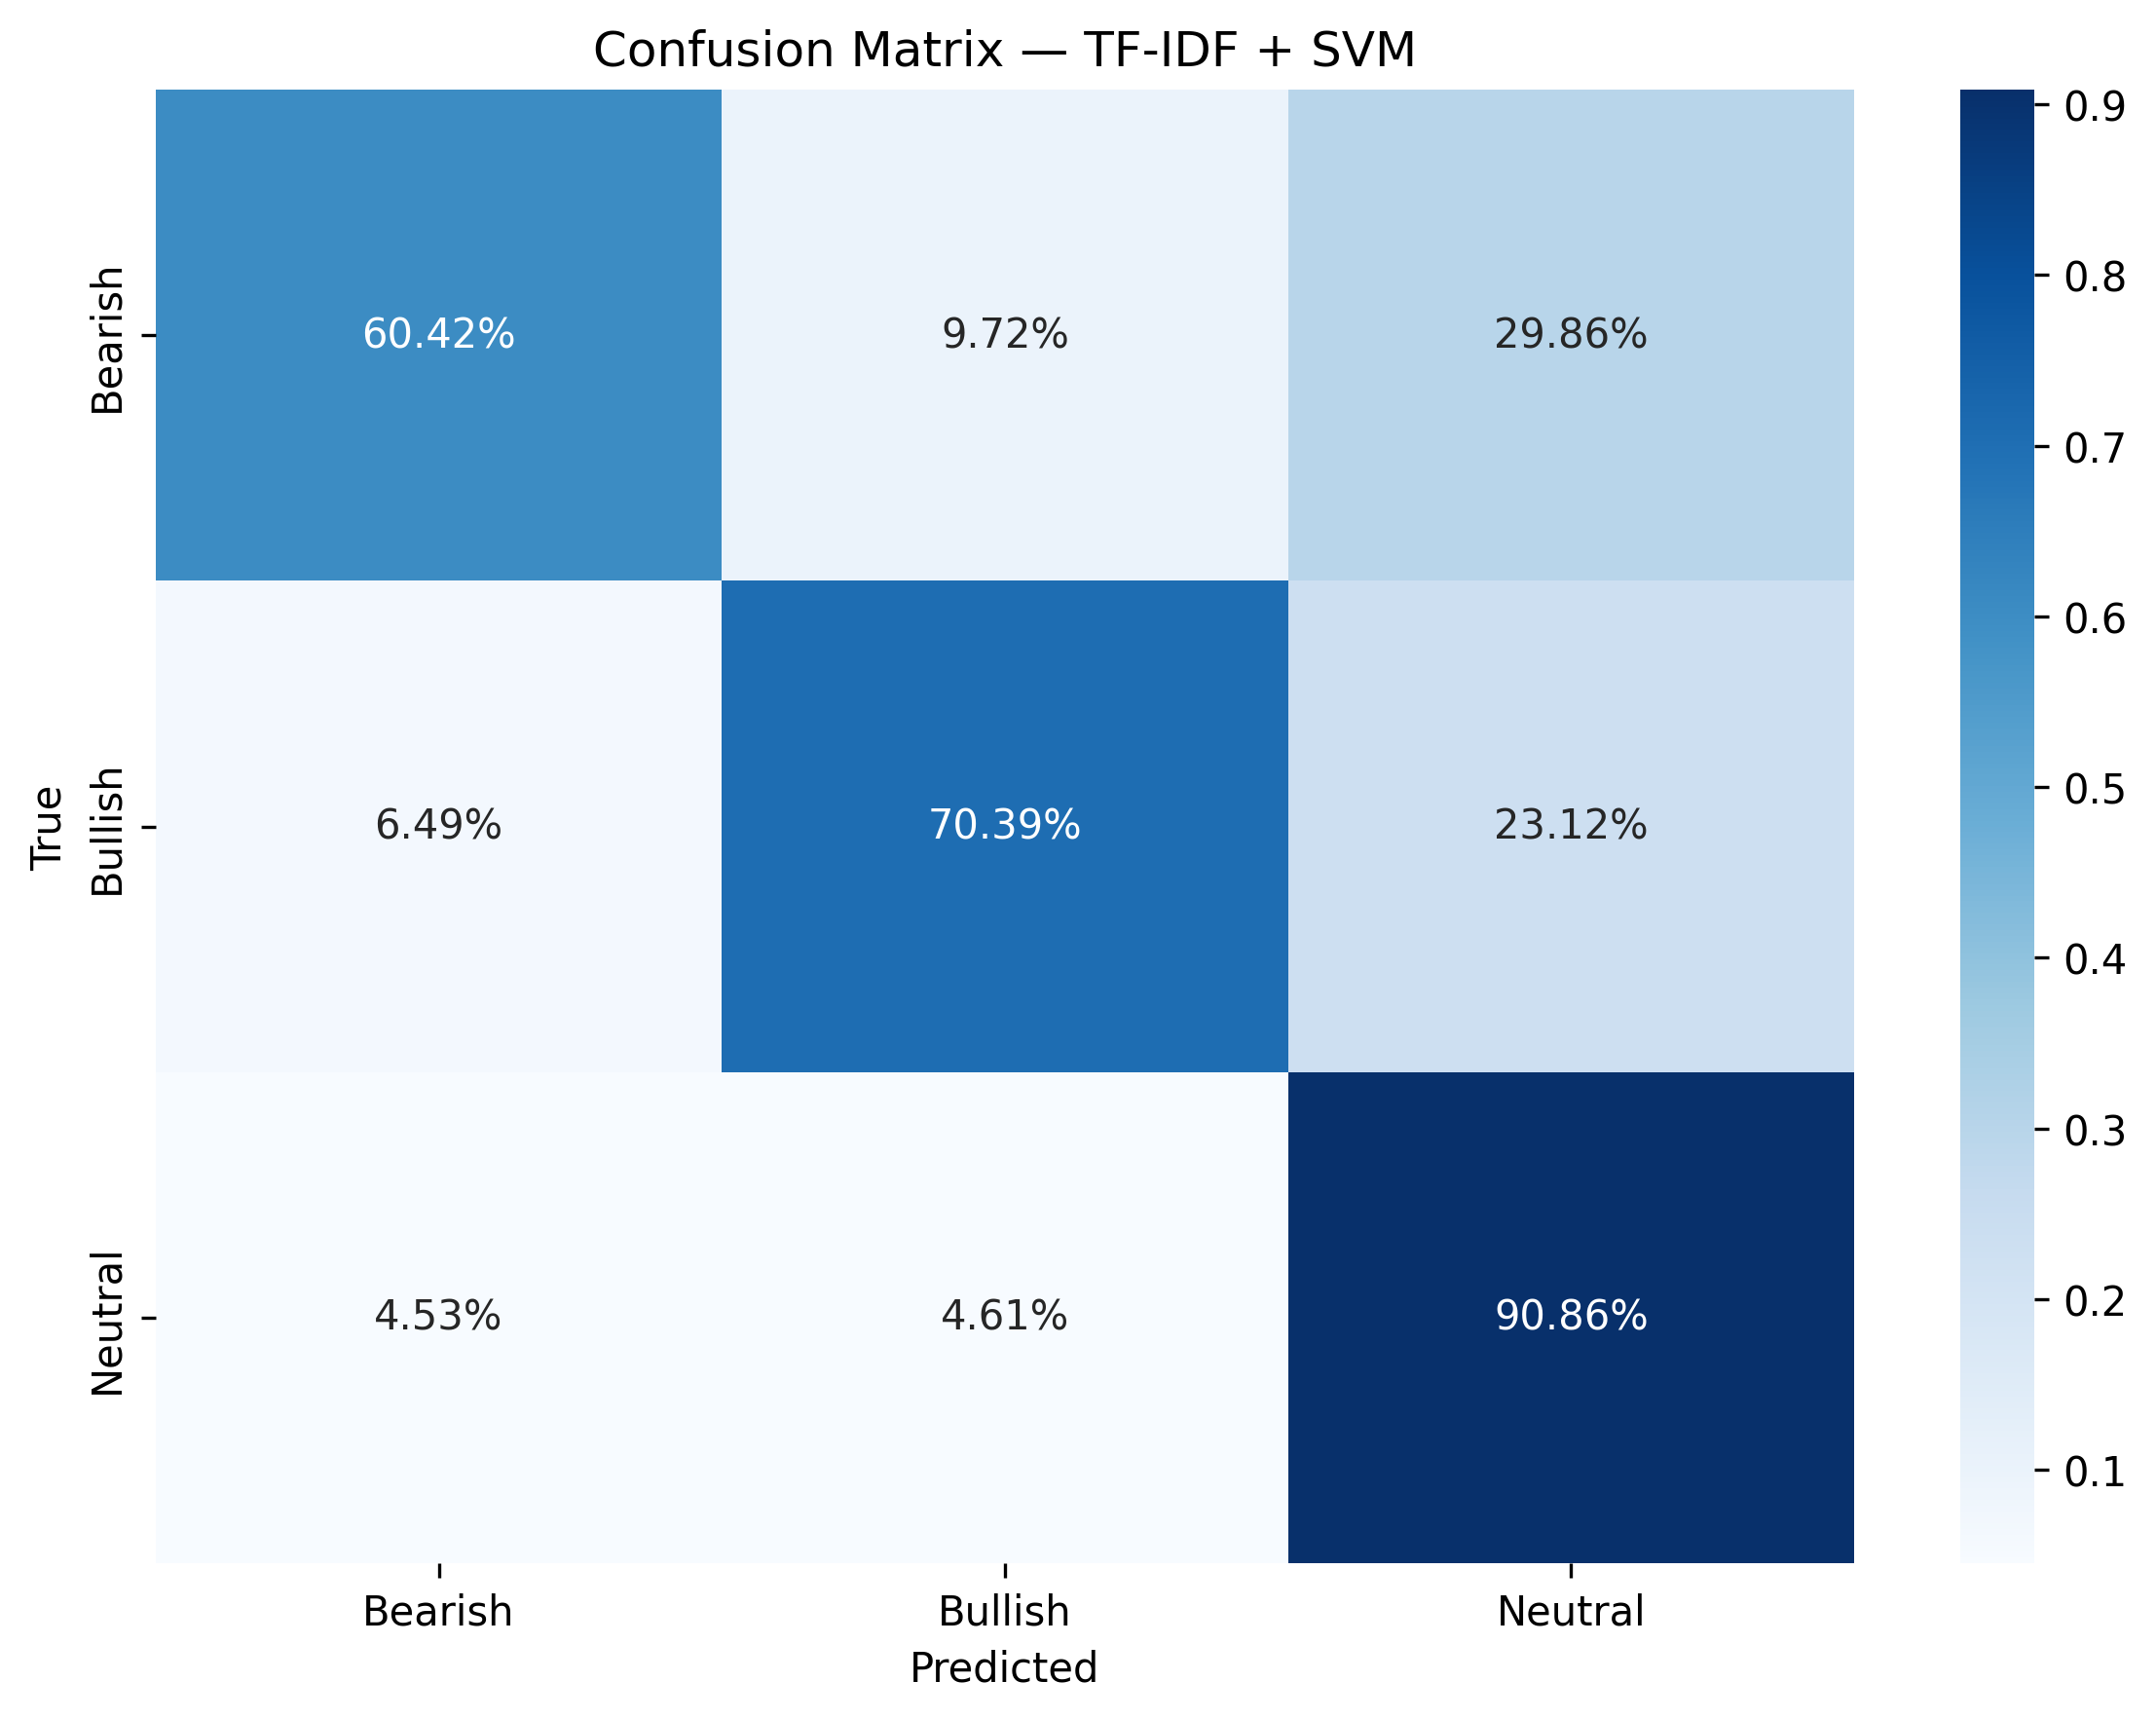
\includegraphics[width=\textwidth]{cm_best_traditional.png}
    \caption{TF-IDF + SVM (best traditional).}
\end{subfigure}
\caption{Confusion matrices for the top models. The dominant error mode is confusion between Neutral and the sentiment classes, while direct Bearish $\leftrightarrow$ Bullish misclassification is rare.}
\label{fig:confusion}
\end{figure}

\subsection{Learning Curve}

\begin{figure}[H]
\centering
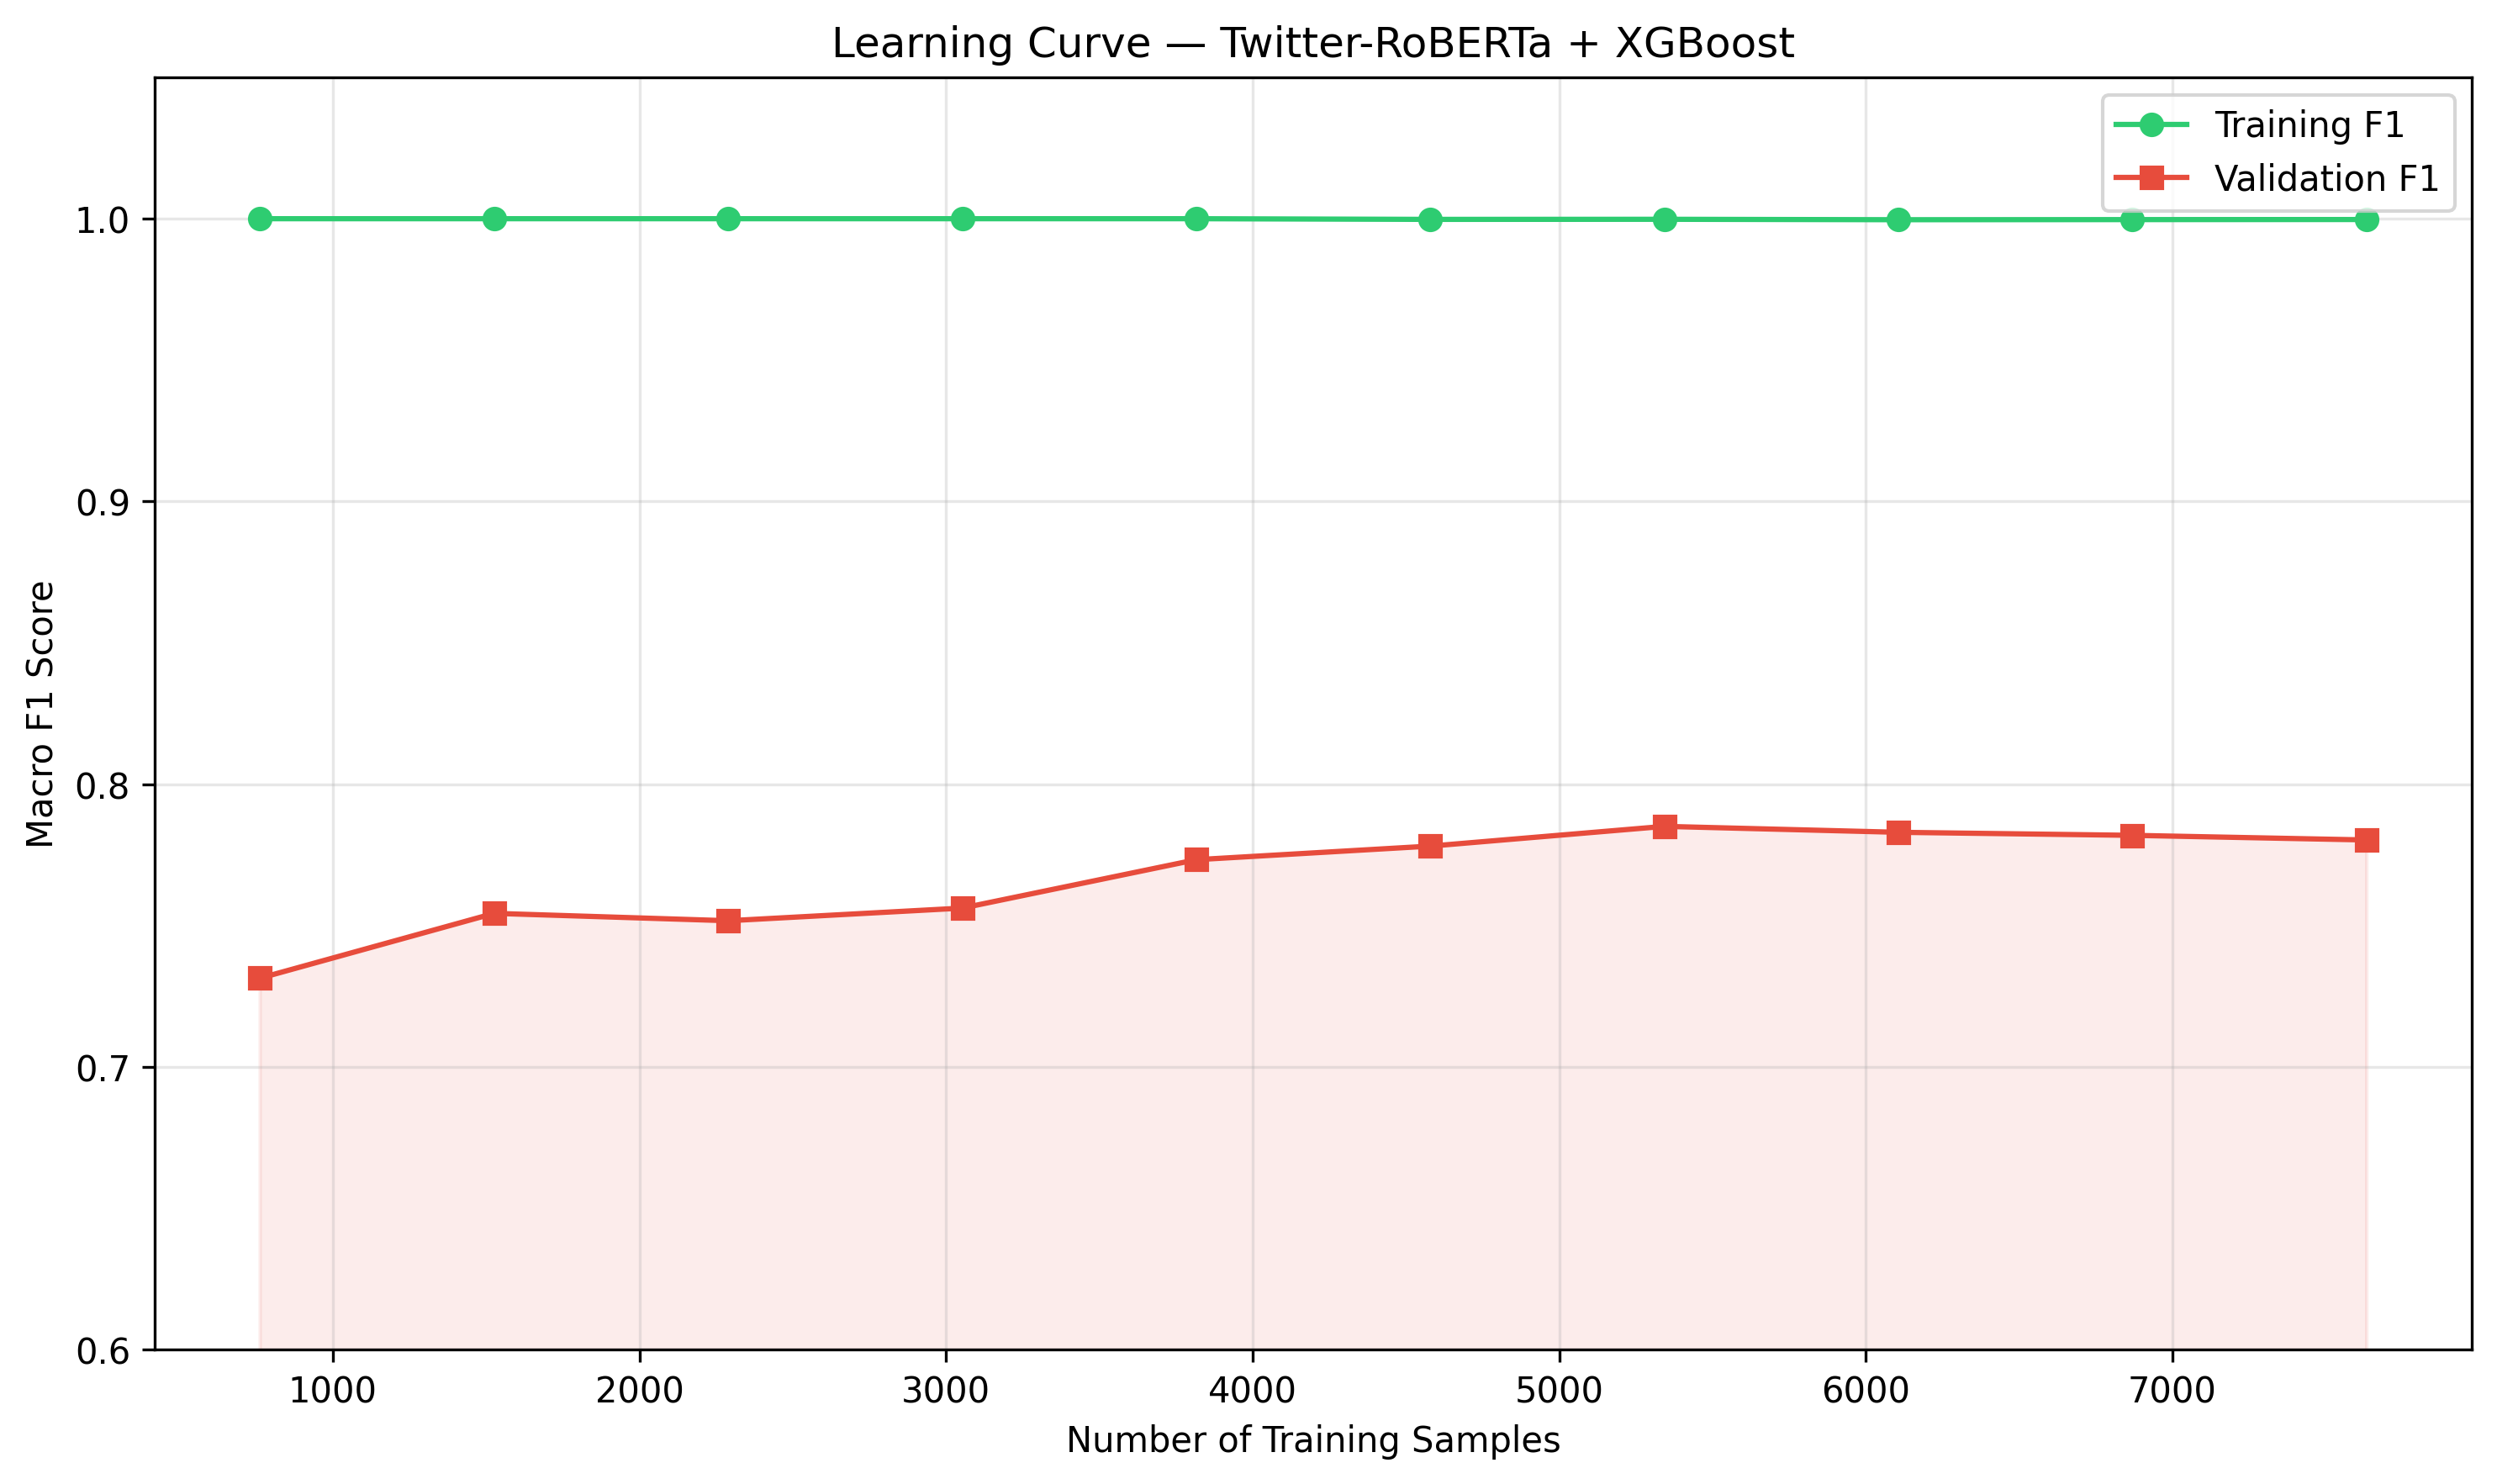
\includegraphics[width=0.78\textwidth]{learning_curve.png}
\caption{Learning curve for Twitter-RoBERTa + XGBoost. Validation F1 grows rapidly from 10\% to 40\% of the data, then plateaus, suggesting the model is approaching its ceiling for this feature representation.}
\label{fig:learning_curve}
\end{figure}

The persistent train--validation gap indicates mild overfitting that more data alone may not resolve --- architectural improvements (e.g., full fine-tuning of the encoder) would be needed to push beyond this ceiling.

\subsection{Statistical Significance}

Paired $t$-tests on the 5-fold CV scores confirm that the performance differences between top models are statistically meaningful:

\begin{itemize}[nosep]
    \item Twitter-RoBERTa + XGBoost vs.\ FinBERT + XGBoost: significant ($p < 0.05$)
    \item Twitter-RoBERTa + XGBoost vs.\ TF-IDF + SVM: significant ($p < 0.05$)
    \item FinBERT + XGBoost vs.\ TF-IDF + SVM: significant ($p < 0.05$)
\end{itemize}

This validates that our model ranking is not an artifact of random variation across folds.

% ============================================================================
% 7. EXTRA WORK
% ============================================================================
\section{Extra Work}

\subsection{Domain-Specific Transformer Encoders}

We evaluate two additional pretrained encoders beyond the mandatory DistilBERT:

\begin{itemize}
    \item \textbf{FinBERT} (\texttt{ProsusAI/finbert}): Trained on financial communications (SEC filings, analyst reports). Achieves 0.779 macro-F1, a \textbf{7.4 percentage point improvement} over DistilBERT, demonstrating the value of financial domain pretraining.
    \item \textbf{Twitter-RoBERTa} (\texttt{cardiffnlp/twitter-roberta-base-sentiment-latest}): Trained on 58 million tweets with sentiment labels. Achieves \textbf{0.794 macro-F1}, the best result overall. The dual domain alignment (Twitter + sentiment) makes this the ideal feature extractor for our task.
\end{itemize}

\subsection{Agentic Workflow}

We implement a \textbf{LangChain-based agent} (\texttt{src/agent.py}) that orchestrates the classification pipeline with five tools:

\begin{enumerate}[nosep]
    \item \textbf{classify\_tweet} --- Classify a single tweet with a specified model.
    \item \textbf{route\_model} --- Intelligent routing based on tweet characteristics (cashtags $\rightarrow$ FinBERT, short tweets with emojis $\rightarrow$ Twitter-RoBERTa).
    \item \textbf{ensemble\_classify} --- Run all models and return majority-vote prediction.
    \item \textbf{compare\_models} --- Display formatted comparison of all model metrics.
    \item \textbf{explain\_prediction} --- Show top contributing features (coefficient-based).
\end{enumerate}

The agent demonstrates non-trivial decision-making: it inspects tweet content to choose the most appropriate model, reconciles disagreements via ensemble voting, and provides human-interpretable explanations. Example transcripts are provided in the \texttt{outputs/} directory.

\subsection{Decoder Model (Attempted)}

We implemented few-shot classification using \textbf{Flan-T5-small}. The prompt provides 2~examples per class and asks the model to output a single digit (0,~1, or~2). However, CPU inference proved infeasible: ${\sim}$2--5~seconds per tweet $\times$ 2,388~test tweets would require over 3~hours. This is documented as a limitation --- GPU access would make this viable.

% ============================================================================
% 8. FINAL PIPELINE
% ============================================================================
\section{Final Pipeline and Predictions}

The production pipeline (\texttt{tm\_final\_42.ipynb}) trains the best model on the \textbf{full training set} (9,543 tweets) and generates predictions for all 2,388 test tweets:

\begin{enumerate}[nosep]
    \item Load and preprocess all data with \texttt{pp\_transformer}.
    \item Extract Twitter-RoBERTa embeddings (cached as \texttt{.npy} files).
    \item Train XGBoost on all 9,543 training embeddings.
    \item Predict on 2,388 test tweets $\rightarrow$ \texttt{pred\_42.csv}.
\end{enumerate}

\begin{table}[H]
\centering
\caption{Test set prediction distribution vs.\ training set distribution.}
\begin{tabular}{lrrrr}
\toprule
\textbf{Class} & \textbf{Pred.\ Count} & \textbf{Pred.\ \%} & \textbf{Train \%} \\
\midrule
Bearish & 309 & 12.9\% & 15.1\% \\
Bullish & 392 & 16.4\% & 20.1\% \\
Neutral & 1,687 & 70.6\% & 64.7\% \\
\bottomrule
\end{tabular}
\end{table}

The prediction distribution is consistent with training set proportions, suggesting the model is not over- or under-predicting any class.

% ============================================================================
% 9. CONCLUSION
% ============================================================================
\section{Conclusion}

\subsection{Summary}

Our systematic evaluation of 32 feature $\times$ classifier combinations reveals that \textbf{domain-specific pretrained Transformer encoders} combined with \textbf{gradient-boosted classifiers} achieve the best results for financial tweet sentiment classification. The winning pipeline --- Twitter-RoBERTa + XGBoost --- achieves \textbf{0.794 macro-F1}, significantly outperforming traditional approaches.

\subsection{Key Takeaways}

\begin{enumerate}
    \item \textbf{Domain alignment $>$ model sophistication}: A general-purpose DistilBERT (66M params) underperforms simple TF-IDF bigrams. A domain-aligned Twitter-RoBERTa (125M params) exceeds both. \textit{What} a model was trained on matters more than \textit{how large} it is.

    \item \textbf{Feature extraction matters more than classifier choice}: The gap between feature families (0.60 for W2V vs.\ 0.79 for Twitter-RoBERTa) far exceeds the gap between classifiers within a family (typically 0.02--0.05).

    \item \textbf{Preprocessing should be conservative}: Aggressive normalization (stopword removal, stemming) destroys sentiment signal. Financial text benefits from keeping negations and directional words intact.

    \item \textbf{Class imbalance handling is essential}: Without balanced class weights, classifiers default to predicting the majority Neutral class, yielding high accuracy but poor minority-class recall.
\end{enumerate}

\subsection{Limitations}

\begin{itemize}[nosep]
    \item \textbf{CPU-only constraint}: Full Transformer fine-tuning was infeasible; frozen embeddings + classifier head is a compromise.
    \item \textbf{No hyperparameter tuning}: Default hyperparameters were used. Grid search could improve results by 1--3\%.
    \item \textbf{Single dataset}: Results may not generalize to other financial text domains (e.g., earnings calls, SEC filings).
    \item \textbf{Decoder model infeasible}: Flan-T5 few-shot classification was too slow on CPU for evaluation.
\end{itemize}

\subsection{Future Work}

\begin{itemize}[nosep]
    \item \textbf{Full fine-tuning with GPU}: Fine-tuning Twitter-RoBERTa's encoder (not just the head) would likely improve results significantly.
    \item \textbf{Ensemble methods}: Combining predictions from multiple feature families could leverage complementary strengths.
    \item \textbf{Temporal analysis}: Financial sentiment may have temporal patterns (market hours vs.\ after-hours) worth exploiting.
    \item \textbf{Hyperparameter optimization}: Bayesian optimization (e.g., Optuna) across the full pipeline.
\end{itemize}

% ============================================================================
% REFERENCES
% ============================================================================
\section*{References}
\addcontentsline{toc}{section}{References}

\begin{enumerate}[nosep, label={[\arabic*]}]
    \item Araci, D. (2019). FinBERT: Financial Sentiment Analysis with Pre-Trained Language Models. \textit{arXiv:1908.10063}.
    \item Barbieri, F., et al. (2020). TweetEval: Unified Benchmark and Comparative Evaluation for Tweet Classification. \textit{arXiv:2010.12421}.
    \item Sanh, V., et al. (2019). DistilBERT, a distilled version of BERT: smaller, faster, cheaper and lighter. \textit{arXiv:1910.01108}.
    \item Chen, T., \& Guestrin, C. (2016). XGBoost: A Scalable Tree Boosting System. \textit{Proceedings of KDD 2016}.
    \item Mikolov, T., et al. (2013). Efficient Estimation of Word Representations in Vector Space. \textit{arXiv:1301.3781}.
    \item Pennington, J., Socher, R., \& Manning, C. D. (2014). GloVe: Global Vectors for Word Representation. \textit{EMNLP 2014}.
    \item Liu, Y., et al. (2019). RoBERTa: A Robustly Optimized BERT Pretraining Approach. \textit{arXiv:1907.11692}.
\end{enumerate}

\end{document}
